\documentclass[11pt]{article}
\usepackage[top=3cm, bottom=3cm, left=3cm, right=3cm]{geometry}

\makeatletter
  \def\input@path{ {sections/} {preamble/} {frontmatter/} {backmatter/} }
  \newcommand*{\version}[1]{\gdef\@version{#1}}
  \newcommand*{\@version}{0.0.0}
  \newcommand*{\manualnr}[1]{\gdef\@manualnr{#1}}
  \newcommand*{\@manualnr}{1}
  \newcommand*{\experiment}[1]{\gdef\@experiment{#1}}
\makeatother

\usepackage{graphicx}
\usepackage{fancyhdr}
\usepackage[printonlyused]{acronym}
\usepackage{wrapfig}
\usepackage{siunitx}
\usepackage[obeyspaces]{url}
\usepackage[table,dvipsnames]{xcolor}
\usepackage[colorlinks=true, linkcolor=darkgray, urlcolor=RoyalBlue, citecolor=RoyalPurple]{hyperref}
\usepackage{fontawesome}
\usepackage{subcaption}
\usepackage{xparse}
\usepackage{ifthen}
\usepackage{multirow}
\usepackage{tabularx}
\usepackage{todonotes}
\usepackage{upgreek}
\usepackage{pdfpages}
% \usepackage[utf8]{inputenc}
\usepackage[T1]{fontenc}
\usepackage{float}
\usepackage{lmodern}
\usepackage{amsmath}
\usepackage[newfloat]{minted}  % display source code
\usepackage[framemethod=TikZ]{mdframed}
\usepackage{tocloft}
\usepackage[nottoc]{tocbibind}
\usepackage{wasysym}

\graphicspath{ {figures/} {figures/main/}}
% ABBREVIATIONS
\newcommand{\z}{\text}
\newcommand{\ar}{\autoref}
\newcommand{\eg}{e.\,g.~}

% UTILS
\newcommand{\cpp}{C\nolinebreak\hspace{-.05em}\raisebox{.4ex}{\tiny\textbf{+}}  \nolinebreak\hspace{-.10em}\raisebox{.4ex}{\tiny\textbf{+}}~}
\newcommand{\code}[1]{{\footnotesize #1}}
\newcommand{\fpath}[1]{\mintinline{control}{#1}}
\newcommand{\mdfsetblack}{\mdfsetup{backgroundcolor=black!75, linecolor=black}}
\newcommand{\mdfsetgrey}{\mdfsetup{backgroundcolor=gray!5, linecolor=black!10}}

% DOCUMENT COMMANDS
\NewDocumentCommand{\caplab}{
  O{} O{} O{}}{\ifthenelse{\equal{#1}{\empty}}{}{\ifthenelse{\equal{#3}{\empty}}{\caption{#1}}{\caption[#3]{#1}}}\ifthenelse{\equal{#2}{\empty}}{}{\label{#2}}}
\newcommand{\pic}[3]{\ifthenelse{\equal{#1}{r}}{\includegraphics[height={#2\linewidth}, angle=-90]{#3}}{\includegraphics[width={#2\linewidth}]{#3}}}
%SUBFIG
\DeclareDocumentCommand{\subfig}{O{.45} O{0} m m O{} O{}}
	{\begin{subfigure}{#1\linewidth}\vspace*{#2\textheight}\centering\includegraphics[height={#3\textheight}]{#4}\caplab[#5][#6]\end{subfigure}}
%SUBFIGS
\DeclareDocumentCommand{\subfigs}{O{fig} m m O{} O{} O{}}{\begin{figure}[ht!]\centering\ifthenelse{\equal{#1}{fig}}{}{#1\hspace*{.05\linewidth}}#2\hspace*{.05\linewidth}#3\caplab[#4][#5][#6]\end{figure}}
% FIG
\DeclareDocumentCommand{\fig}{O{n} m m O{} O{} O{}}{\begin{figure}[ht!]\centering\pic{#1}{#2}{#3}\caplab[#4][#5][#6]\end{figure}}
% WRAPFIG
\DeclareDocumentCommand{\wrapfig}{O{l} m m O{} O{} O{}}{
	\begin{wrapfigure}{#1}{#2\linewidth}\includegraphics[width={.95\linewidth}]{#3}\caplab[#4][#5][#6]\end{wrapfigure}}
% NICETAB
\DeclareDocumentCommand{\nicetab}{O{} m m O{} O{} O{}}{
  \begin{table}[ht!]#1\centering \begin{tabular}
    {#2}\noalign{\hrule height 1.3pt}#3
    \noalign{\hrule height 1.3pt}
  \end{tabular}\caplab[#4][#5][#6]\end{table}}

% TITLEPAGE
\makeatletter
\renewcommand*{\maketitle}{
\begin{titlepage}
%
  \begin{figure}
    \begin{minipage}{0.45\linewidth}\flushleft
      
\includegraphics[height=.16\textheight]{VPLogo}\vspace*{2ex}
    \end{minipage}
    \hfill
    \begin{minipage}{0.45\linewidth}\flushright\vspace*{6ex}
      
\includegraphics[height=.026\textheight]{LogoDPHYS}\\[3ex]
      Version \@version\\
      Manual Number: \@manualnr\\[0.3cm]
    \end{minipage}
    \hrule height 1pt
  \end{figure}\vspace*{.4cm}
%
  \centering
  {\Large\scshape Instruction Manual\strut\par}\vspace*{.5cm}
  {\Huge\bfseries Advanced Physics Lab\unskip\strut\par}\vspace*{.3cm}
  {\Huge\bfseries\@experiment\unskip\strut\par}\vspace*{1.3cm}
  {\huge\itshape\@title\strut\par}\vspace*{1.3cm}
  {\large\@author\unskip\strut\par}\vspace*{.5cm}
  \begin{abstract}
%
The experiment ``Electronic Analog+Digital'' provides an introduction into modern data taking by reading out analog sensors and control devices with an ATmega328P micro-controller using the Arduino Uno platform. This manual will introduce you to the Arduino board and programming, the installation of the required software and the electrical components you will have to use. Basic knowledge on electronics, how to use oscilloscopes, bread boards and power supplies is recommended. \par
%
During the experiment you will learn how to build a circuit required for measuring the temperature with an NTC, including an operational amplifier. Furthermore you will control a fans speed via pulse width modulation and can build a regulator to keep the temperature of an object constant. Eventually you will use the Arduino to build a PID controller, which is a widely used technique.\par
%
In case you should already have previous knowledge we will provide additional components you can use in your experiment. Own ideas for other applications of the Arduino are very welcome and can be built after consulting the assistants.
%
\end{abstract}

  \vfill
%
  \flushleft
  ETH Z\"urich, Switzerland, \@date
%
\end{titlepage}}







\sisetup{detect-weight=true, detect-family=true, range-units=single, range-phrase=$\ \sim\ $, separate-uncertainty=true}

%\newfontfamily\ubuntu{Ubuntu}
%\newfontfamily\dejavu{DejaVuSans}

\setlength{\headheight}{14pt}

%%%%%%%%%%%%%%%%%%%%%%%%%%%%%%%%%%%%%%%%%%%%%%%%%%%%%%%%%%%%%%%%%%%%%%%%%%%%%%%% 
%%% ~ Arduino Language - Arduino IDE Colors ~                                  %%%
%%%                                                                            %%%
%%% Kyle Rocha-Brownell | 10/2/2017 | No Licence                               %%%
%%% -------------------------------------------------------------------------- %%%
%%%                                                                            %%%
%%% Place this file in your working directory (next to the latex file you're   %%%
%%% working on).  To add it to your project, place:                            %%%
%%%    %%%%%%%%%%%%%%%%%%%%%%%%%%%%%%%%%%%%%%%%%%%%%%%%%%%%%%%%%%%%%%%%%%%%%%%%%%%%%%%% 
%%% ~ Arduino Language - Arduino IDE Colors ~                                  %%%
%%%                                                                            %%%
%%% Kyle Rocha-Brownell | 10/2/2017 | No Licence                               %%%
%%% -------------------------------------------------------------------------- %%%
%%%                                                                            %%%
%%% Place this file in your working directory (next to the latex file you're   %%%
%%% working on).  To add it to your project, place:                            %%%
%%%    %%%%%%%%%%%%%%%%%%%%%%%%%%%%%%%%%%%%%%%%%%%%%%%%%%%%%%%%%%%%%%%%%%%%%%%%%%%%%%%% 
%%% ~ Arduino Language - Arduino IDE Colors ~                                  %%%
%%%                                                                            %%%
%%% Kyle Rocha-Brownell | 10/2/2017 | No Licence                               %%%
%%% -------------------------------------------------------------------------- %%%
%%%                                                                            %%%
%%% Place this file in your working directory (next to the latex file you're   %%%
%%% working on).  To add it to your project, place:                            %%%
%%%    \input{arduinoLanguage.tex}                                             %%%
%%% somewhere before \begin{document} in your latex file.                      %%%
%%%                                                                            %%%
%%% In your document, place your arduino code between:                         %%%
%%%   \begin{lstlisting}[language=Arduino]                                     %%%
%%% and:                                                                       %%%
%%%   \end{lstlisting}                                                         %%%
%%%                                                                            %%%
%%% Or create your own style to add non-built-in functions and variables.      %%%
%%%                                                                            %%%
 %%%%%%%%%%%%%%%%%%%%%%%%%%%%%%%%%%%%%%%%%%%%%%%%%%%%%%%%%%%%%%%%%%%%%%%%%%%%%%%% 

\usepackage{color}
\usepackage{listings}    
\usepackage{courier}

%%% Define Custom IDE Colors %%%
\definecolor{arduinoGreen}    {rgb} {0.17, 0.43, 0.01}
\definecolor{arduinoGrey}     {rgb} {0.47, 0.47, 0.33}
\definecolor{arduinoOrange}   {rgb} {0.8 , 0.4 , 0   }
\definecolor{arduinoBlue}     {rgb} {0.01, 0.61, 0.98}
\definecolor{arduinoDarkBlue} {rgb} {0.0 , 0.2 , 0.5 }

%%% Define Arduino Language %%%
\lstdefinelanguage{Arduino}{
  language=C++, % begin with default C++ settings 
%
%
  %%% Keyword Color Group 1 %%%  (called KEYWORD3 by arduino)
  keywordstyle=\color{arduinoGreen},   
  deletekeywords={  % remove all arduino keywords that might be in c++
                break, case, override, final, continue, default, do, else, for, 
                if, return, goto, switch, throw, try, while, setup, loop, export, 
                not, or, and, xor, include, define, elif, else, error, if, ifdef, 
                ifndef, pragma, warning,
                HIGH, LOW, INPUT, INPUT_PULLUP, OUTPUT, DEC, BIN, HEX, OCT, PI, 
                HALF_PI, TWO_PI, LSBFIRST, MSBFIRST, CHANGE, FALLING, RISING, 
                DEFAULT, EXTERNAL, INTERNAL, INTERNAL1V1, INTERNAL2V56, LED_BUILTIN, 
                LED_BUILTIN_RX, LED_BUILTIN_TX, DIGITAL_MESSAGE, FIRMATA_STRING, 
                ANALOG_MESSAGE, REPORT_DIGITAL, REPORT_ANALOG, SET_PIN_MODE, 
                SYSTEM_RESET, SYSEX_START, auto, int8_t, int16_t, int32_t, int64_t, 
                uint8_t, uint16_t, uint32_t, uint64_t, char16_t, char32_t, operator, 
                enum, delete, bool, boolean, byte, char, const, false, float, double, 
                null, NULL, int, long, new, private, protected, public, short, 
                signed, static, volatile, String, void, true, unsigned, word, array, 
                sizeof, dynamic_cast, typedef, const_cast, struct, static_cast, union, 
                friend, extern, class, reinterpret_cast, register, explicit, inline, 
                _Bool, complex, _Complex, _Imaginary, atomic_bool, atomic_char, 
                atomic_schar, atomic_uchar, atomic_short, atomic_ushort, atomic_int, 
                atomic_uint, atomic_long, atomic_ulong, atomic_llong, atomic_ullong, 
                virtual, PROGMEM,
                Serial, Serial1, Serial2, Serial3, SerialUSB, Keyboard, Mouse,
                abs, acos, asin, atan, atan2, ceil, constrain, cos, degrees, exp, 
                floor, log, map, max, min, radians, random, randomSeed, round, sin, 
                sq, sqrt, tan, pow, bitRead, bitWrite, bitSet, bitClear, bit, 
                highByte, lowByte, analogReference, analogRead, 
                analogReadResolution, analogWrite, analogWriteResolution, 
                attachInterrupt, detachInterrupt, digitalPinToInterrupt, delay, 
                delayMicroseconds, digitalWrite, digitalRead, interrupts, millis, 
                micros, noInterrupts, noTone, pinMode, pulseIn, pulseInLong, shiftIn, 
                shiftOut, tone, yield, Stream, begin, end, peek, read, print, 
                println, available, availableForWrite, flush, setTimeout, find, 
                findUntil, parseInt, parseFloat, readBytes, readBytesUntil, readString, 
                readStringUntil, trim, toUpperCase, toLowerCase, charAt, compareTo, 
                concat, endsWith, startsWith, equals, equalsIgnoreCase, getBytes, 
                indexOf, lastIndexOf, length, replace, setCharAt, substring, 
                toCharArray, toInt, press, release, releaseAll, accept, click, move, 
                isPressed, isAlphaNumeric, isAlpha, isAscii, isWhitespace, isControl, 
                isDigit, isGraph, isLowerCase, isPrintable, isPunct, isSpace, 
                isUpperCase, isHexadecimalDigit, 
                }, 
  morekeywords={   % add arduino structures to group 1
                break, case, override, final, continue, default, do, else, for, 
                if, return, goto, switch, throw, try, while, setup, loop, export, 
                not, or, and, xor, include, define, elif, else, error, if, ifdef, 
                ifndef, pragma, warning,
                }, 
% 
%
  %%% Keyword Color Group 2 %%%  (called LITERAL1 by arduino)
  keywordstyle=[2]\color{arduinoBlue},   
  keywords=[2]{   % add variables and dataTypes as 2nd group  
                HIGH, LOW, INPUT, INPUT_PULLUP, OUTPUT, DEC, BIN, HEX, OCT, PI, 
                HALF_PI, TWO_PI, LSBFIRST, MSBFIRST, CHANGE, FALLING, RISING, 
                DEFAULT, EXTERNAL, INTERNAL, INTERNAL1V1, INTERNAL2V56, LED_BUILTIN, 
                LED_BUILTIN_RX, LED_BUILTIN_TX, DIGITAL_MESSAGE, FIRMATA_STRING, 
                ANALOG_MESSAGE, REPORT_DIGITAL, REPORT_ANALOG, SET_PIN_MODE, 
                SYSTEM_RESET, SYSEX_START, auto, int8_t, int16_t, int32_t, int64_t, 
                uint8_t, uint16_t, uint32_t, uint64_t, char16_t, char32_t, operator, 
                enum, delete, bool, boolean, byte, char, const, false, float, double, 
                null, NULL, int, long, new, private, protected, public, short, 
                signed, static, volatile, String, void, true, unsigned, word, array, 
                sizeof, dynamic_cast, typedef, const_cast, struct, static_cast, union, 
                friend, extern, class, reinterpret_cast, register, explicit, inline, 
                _Bool, complex, _Complex, _Imaginary, atomic_bool, atomic_char, 
                atomic_schar, atomic_uchar, atomic_short, atomic_ushort, atomic_int, 
                atomic_uint, atomic_long, atomic_ulong, atomic_llong, atomic_ullong, 
                virtual, PROGMEM,
                },  
% 
%
  %%% Keyword Color Group 3 %%%  (called KEYWORD1 by arduino)
  keywordstyle=[3]\bfseries\color{arduinoOrange},
  keywords=[3]{  % add built-in functions as a 3rd group
                Serial, Serial1, Serial2, Serial3, SerialUSB, Keyboard, Mouse,
                },      
%
%
  %%% Keyword Color Group 4 %%%  (called KEYWORD2 by arduino)
  keywordstyle=[4]\color{arduinoOrange},
  keywords=[4]{  % add more built-in functions as a 4th group
                abs, acos, asin, atan, atan2, ceil, constrain, cos, degrees, exp, 
                floor, log, map, max, min, radians, random, randomSeed, round, sin, 
                sq, sqrt, tan, pow, bitRead, bitWrite, bitSet, bitClear, bit, 
                highByte, lowByte, analogReference, analogRead, 
                analogReadResolution, analogWrite, analogWriteResolution, 
                attachInterrupt, detachInterrupt, digitalPinToInterrupt, delay, 
                delayMicroseconds, digitalWrite, digitalRead, interrupts, millis, 
                micros, noInterrupts, noTone, pinMode, pulseIn, pulseInLong, shiftIn, 
                shiftOut, tone, yield, Stream, begin, end, peek, read, print, 
                println, available, availableForWrite, flush, setTimeout, find, 
                findUntil, parseInt, parseFloat, readBytes, readBytesUntil, readString, 
                readStringUntil, trim, toUpperCase, toLowerCase, charAt, compareTo, 
                concat, endsWith, startsWith, equals, equalsIgnoreCase, getBytes, 
                indexOf, lastIndexOf, length, replace, setCharAt, substring, 
                toCharArray, toInt, press, release, releaseAll, accept, click, move, 
                isPressed, isAlphaNumeric, isAlpha, isAscii, isWhitespace, isControl, 
                isDigit, isGraph, isLowerCase, isPrintable, isPunct, isSpace, 
                isUpperCase, isHexadecimalDigit, 
                },      
%
%
  %%% Set Other Colors %%%
  stringstyle=\color{arduinoDarkBlue},    
  commentstyle=\color{arduinoGrey},    
%          
%   
  %%%% Line Numbering %%%%
   numbers=left,                    
  numbersep=5pt,                   
  numberstyle=\color{arduinoGrey},    
  %stepnumber=2,                      % show every 2 line numbers
%
%
  %%%% Code Box Style %%%%
  breaklines=true,                    % wordwrapping
  tabsize=2,         
  basicstyle=\ttfamily  
}                                             %%%
%%% somewhere before \begin{document} in your latex file.                      %%%
%%%                                                                            %%%
%%% In your document, place your arduino code between:                         %%%
%%%   \begin{lstlisting}[language=Arduino]                                     %%%
%%% and:                                                                       %%%
%%%   \end{lstlisting}                                                         %%%
%%%                                                                            %%%
%%% Or create your own style to add non-built-in functions and variables.      %%%
%%%                                                                            %%%
 %%%%%%%%%%%%%%%%%%%%%%%%%%%%%%%%%%%%%%%%%%%%%%%%%%%%%%%%%%%%%%%%%%%%%%%%%%%%%%%% 

\usepackage{color}
\usepackage{listings}    
\usepackage{courier}

%%% Define Custom IDE Colors %%%
\definecolor{arduinoGreen}    {rgb} {0.17, 0.43, 0.01}
\definecolor{arduinoGrey}     {rgb} {0.47, 0.47, 0.33}
\definecolor{arduinoOrange}   {rgb} {0.8 , 0.4 , 0   }
\definecolor{arduinoBlue}     {rgb} {0.01, 0.61, 0.98}
\definecolor{arduinoDarkBlue} {rgb} {0.0 , 0.2 , 0.5 }

%%% Define Arduino Language %%%
\lstdefinelanguage{Arduino}{
  language=C++, % begin with default C++ settings 
%
%
  %%% Keyword Color Group 1 %%%  (called KEYWORD3 by arduino)
  keywordstyle=\color{arduinoGreen},   
  deletekeywords={  % remove all arduino keywords that might be in c++
                break, case, override, final, continue, default, do, else, for, 
                if, return, goto, switch, throw, try, while, setup, loop, export, 
                not, or, and, xor, include, define, elif, else, error, if, ifdef, 
                ifndef, pragma, warning,
                HIGH, LOW, INPUT, INPUT_PULLUP, OUTPUT, DEC, BIN, HEX, OCT, PI, 
                HALF_PI, TWO_PI, LSBFIRST, MSBFIRST, CHANGE, FALLING, RISING, 
                DEFAULT, EXTERNAL, INTERNAL, INTERNAL1V1, INTERNAL2V56, LED_BUILTIN, 
                LED_BUILTIN_RX, LED_BUILTIN_TX, DIGITAL_MESSAGE, FIRMATA_STRING, 
                ANALOG_MESSAGE, REPORT_DIGITAL, REPORT_ANALOG, SET_PIN_MODE, 
                SYSTEM_RESET, SYSEX_START, auto, int8_t, int16_t, int32_t, int64_t, 
                uint8_t, uint16_t, uint32_t, uint64_t, char16_t, char32_t, operator, 
                enum, delete, bool, boolean, byte, char, const, false, float, double, 
                null, NULL, int, long, new, private, protected, public, short, 
                signed, static, volatile, String, void, true, unsigned, word, array, 
                sizeof, dynamic_cast, typedef, const_cast, struct, static_cast, union, 
                friend, extern, class, reinterpret_cast, register, explicit, inline, 
                _Bool, complex, _Complex, _Imaginary, atomic_bool, atomic_char, 
                atomic_schar, atomic_uchar, atomic_short, atomic_ushort, atomic_int, 
                atomic_uint, atomic_long, atomic_ulong, atomic_llong, atomic_ullong, 
                virtual, PROGMEM,
                Serial, Serial1, Serial2, Serial3, SerialUSB, Keyboard, Mouse,
                abs, acos, asin, atan, atan2, ceil, constrain, cos, degrees, exp, 
                floor, log, map, max, min, radians, random, randomSeed, round, sin, 
                sq, sqrt, tan, pow, bitRead, bitWrite, bitSet, bitClear, bit, 
                highByte, lowByte, analogReference, analogRead, 
                analogReadResolution, analogWrite, analogWriteResolution, 
                attachInterrupt, detachInterrupt, digitalPinToInterrupt, delay, 
                delayMicroseconds, digitalWrite, digitalRead, interrupts, millis, 
                micros, noInterrupts, noTone, pinMode, pulseIn, pulseInLong, shiftIn, 
                shiftOut, tone, yield, Stream, begin, end, peek, read, print, 
                println, available, availableForWrite, flush, setTimeout, find, 
                findUntil, parseInt, parseFloat, readBytes, readBytesUntil, readString, 
                readStringUntil, trim, toUpperCase, toLowerCase, charAt, compareTo, 
                concat, endsWith, startsWith, equals, equalsIgnoreCase, getBytes, 
                indexOf, lastIndexOf, length, replace, setCharAt, substring, 
                toCharArray, toInt, press, release, releaseAll, accept, click, move, 
                isPressed, isAlphaNumeric, isAlpha, isAscii, isWhitespace, isControl, 
                isDigit, isGraph, isLowerCase, isPrintable, isPunct, isSpace, 
                isUpperCase, isHexadecimalDigit, 
                }, 
  morekeywords={   % add arduino structures to group 1
                break, case, override, final, continue, default, do, else, for, 
                if, return, goto, switch, throw, try, while, setup, loop, export, 
                not, or, and, xor, include, define, elif, else, error, if, ifdef, 
                ifndef, pragma, warning,
                }, 
% 
%
  %%% Keyword Color Group 2 %%%  (called LITERAL1 by arduino)
  keywordstyle=[2]\color{arduinoBlue},   
  keywords=[2]{   % add variables and dataTypes as 2nd group  
                HIGH, LOW, INPUT, INPUT_PULLUP, OUTPUT, DEC, BIN, HEX, OCT, PI, 
                HALF_PI, TWO_PI, LSBFIRST, MSBFIRST, CHANGE, FALLING, RISING, 
                DEFAULT, EXTERNAL, INTERNAL, INTERNAL1V1, INTERNAL2V56, LED_BUILTIN, 
                LED_BUILTIN_RX, LED_BUILTIN_TX, DIGITAL_MESSAGE, FIRMATA_STRING, 
                ANALOG_MESSAGE, REPORT_DIGITAL, REPORT_ANALOG, SET_PIN_MODE, 
                SYSTEM_RESET, SYSEX_START, auto, int8_t, int16_t, int32_t, int64_t, 
                uint8_t, uint16_t, uint32_t, uint64_t, char16_t, char32_t, operator, 
                enum, delete, bool, boolean, byte, char, const, false, float, double, 
                null, NULL, int, long, new, private, protected, public, short, 
                signed, static, volatile, String, void, true, unsigned, word, array, 
                sizeof, dynamic_cast, typedef, const_cast, struct, static_cast, union, 
                friend, extern, class, reinterpret_cast, register, explicit, inline, 
                _Bool, complex, _Complex, _Imaginary, atomic_bool, atomic_char, 
                atomic_schar, atomic_uchar, atomic_short, atomic_ushort, atomic_int, 
                atomic_uint, atomic_long, atomic_ulong, atomic_llong, atomic_ullong, 
                virtual, PROGMEM,
                },  
% 
%
  %%% Keyword Color Group 3 %%%  (called KEYWORD1 by arduino)
  keywordstyle=[3]\bfseries\color{arduinoOrange},
  keywords=[3]{  % add built-in functions as a 3rd group
                Serial, Serial1, Serial2, Serial3, SerialUSB, Keyboard, Mouse,
                },      
%
%
  %%% Keyword Color Group 4 %%%  (called KEYWORD2 by arduino)
  keywordstyle=[4]\color{arduinoOrange},
  keywords=[4]{  % add more built-in functions as a 4th group
                abs, acos, asin, atan, atan2, ceil, constrain, cos, degrees, exp, 
                floor, log, map, max, min, radians, random, randomSeed, round, sin, 
                sq, sqrt, tan, pow, bitRead, bitWrite, bitSet, bitClear, bit, 
                highByte, lowByte, analogReference, analogRead, 
                analogReadResolution, analogWrite, analogWriteResolution, 
                attachInterrupt, detachInterrupt, digitalPinToInterrupt, delay, 
                delayMicroseconds, digitalWrite, digitalRead, interrupts, millis, 
                micros, noInterrupts, noTone, pinMode, pulseIn, pulseInLong, shiftIn, 
                shiftOut, tone, yield, Stream, begin, end, peek, read, print, 
                println, available, availableForWrite, flush, setTimeout, find, 
                findUntil, parseInt, parseFloat, readBytes, readBytesUntil, readString, 
                readStringUntil, trim, toUpperCase, toLowerCase, charAt, compareTo, 
                concat, endsWith, startsWith, equals, equalsIgnoreCase, getBytes, 
                indexOf, lastIndexOf, length, replace, setCharAt, substring, 
                toCharArray, toInt, press, release, releaseAll, accept, click, move, 
                isPressed, isAlphaNumeric, isAlpha, isAscii, isWhitespace, isControl, 
                isDigit, isGraph, isLowerCase, isPrintable, isPunct, isSpace, 
                isUpperCase, isHexadecimalDigit, 
                },      
%
%
  %%% Set Other Colors %%%
  stringstyle=\color{arduinoDarkBlue},    
  commentstyle=\color{arduinoGrey},    
%          
%   
  %%%% Line Numbering %%%%
   numbers=left,                    
  numbersep=5pt,                   
  numberstyle=\color{arduinoGrey},    
  %stepnumber=2,                      % show every 2 line numbers
%
%
  %%%% Code Box Style %%%%
  breaklines=true,                    % wordwrapping
  tabsize=2,         
  basicstyle=\ttfamily  
}                                             %%%
%%% somewhere before \begin{document} in your latex file.                      %%%
%%%                                                                            %%%
%%% In your document, place your arduino code between:                         %%%
%%%   \begin{lstlisting}[language=Arduino]                                     %%%
%%% and:                                                                       %%%
%%%   \end{lstlisting}                                                         %%%
%%%                                                                            %%%
%%% Or create your own style to add non-built-in functions and variables.      %%%
%%%                                                                            %%%
 %%%%%%%%%%%%%%%%%%%%%%%%%%%%%%%%%%%%%%%%%%%%%%%%%%%%%%%%%%%%%%%%%%%%%%%%%%%%%%%% 

\usepackage{color}
\usepackage{listings}    
\usepackage{courier}

%%% Define Custom IDE Colors %%%
\definecolor{arduinoGreen}    {rgb} {0.17, 0.43, 0.01}
\definecolor{arduinoGrey}     {rgb} {0.47, 0.47, 0.33}
\definecolor{arduinoOrange}   {rgb} {0.8 , 0.4 , 0   }
\definecolor{arduinoBlue}     {rgb} {0.01, 0.61, 0.98}
\definecolor{arduinoDarkBlue} {rgb} {0.0 , 0.2 , 0.5 }

%%% Define Arduino Language %%%
\lstdefinelanguage{Arduino}{
  language=C++, % begin with default C++ settings 
%
%
  %%% Keyword Color Group 1 %%%  (called KEYWORD3 by arduino)
  keywordstyle=\color{arduinoGreen},   
  deletekeywords={  % remove all arduino keywords that might be in c++
                break, case, override, final, continue, default, do, else, for, 
                if, return, goto, switch, throw, try, while, setup, loop, export, 
                not, or, and, xor, include, define, elif, else, error, if, ifdef, 
                ifndef, pragma, warning,
                HIGH, LOW, INPUT, INPUT_PULLUP, OUTPUT, DEC, BIN, HEX, OCT, PI, 
                HALF_PI, TWO_PI, LSBFIRST, MSBFIRST, CHANGE, FALLING, RISING, 
                DEFAULT, EXTERNAL, INTERNAL, INTERNAL1V1, INTERNAL2V56, LED_BUILTIN, 
                LED_BUILTIN_RX, LED_BUILTIN_TX, DIGITAL_MESSAGE, FIRMATA_STRING, 
                ANALOG_MESSAGE, REPORT_DIGITAL, REPORT_ANALOG, SET_PIN_MODE, 
                SYSTEM_RESET, SYSEX_START, auto, int8_t, int16_t, int32_t, int64_t, 
                uint8_t, uint16_t, uint32_t, uint64_t, char16_t, char32_t, operator, 
                enum, delete, bool, boolean, byte, char, const, false, float, double, 
                null, NULL, int, long, new, private, protected, public, short, 
                signed, static, volatile, String, void, true, unsigned, word, array, 
                sizeof, dynamic_cast, typedef, const_cast, struct, static_cast, union, 
                friend, extern, class, reinterpret_cast, register, explicit, inline, 
                _Bool, complex, _Complex, _Imaginary, atomic_bool, atomic_char, 
                atomic_schar, atomic_uchar, atomic_short, atomic_ushort, atomic_int, 
                atomic_uint, atomic_long, atomic_ulong, atomic_llong, atomic_ullong, 
                virtual, PROGMEM,
                Serial, Serial1, Serial2, Serial3, SerialUSB, Keyboard, Mouse,
                abs, acos, asin, atan, atan2, ceil, constrain, cos, degrees, exp, 
                floor, log, map, max, min, radians, random, randomSeed, round, sin, 
                sq, sqrt, tan, pow, bitRead, bitWrite, bitSet, bitClear, bit, 
                highByte, lowByte, analogReference, analogRead, 
                analogReadResolution, analogWrite, analogWriteResolution, 
                attachInterrupt, detachInterrupt, digitalPinToInterrupt, delay, 
                delayMicroseconds, digitalWrite, digitalRead, interrupts, millis, 
                micros, noInterrupts, noTone, pinMode, pulseIn, pulseInLong, shiftIn, 
                shiftOut, tone, yield, Stream, begin, end, peek, read, print, 
                println, available, availableForWrite, flush, setTimeout, find, 
                findUntil, parseInt, parseFloat, readBytes, readBytesUntil, readString, 
                readStringUntil, trim, toUpperCase, toLowerCase, charAt, compareTo, 
                concat, endsWith, startsWith, equals, equalsIgnoreCase, getBytes, 
                indexOf, lastIndexOf, length, replace, setCharAt, substring, 
                toCharArray, toInt, press, release, releaseAll, accept, click, move, 
                isPressed, isAlphaNumeric, isAlpha, isAscii, isWhitespace, isControl, 
                isDigit, isGraph, isLowerCase, isPrintable, isPunct, isSpace, 
                isUpperCase, isHexadecimalDigit, 
                }, 
  morekeywords={   % add arduino structures to group 1
                break, case, override, final, continue, default, do, else, for, 
                if, return, goto, switch, throw, try, while, setup, loop, export, 
                not, or, and, xor, include, define, elif, else, error, if, ifdef, 
                ifndef, pragma, warning,
                }, 
% 
%
  %%% Keyword Color Group 2 %%%  (called LITERAL1 by arduino)
  keywordstyle=[2]\color{arduinoBlue},   
  keywords=[2]{   % add variables and dataTypes as 2nd group  
                HIGH, LOW, INPUT, INPUT_PULLUP, OUTPUT, DEC, BIN, HEX, OCT, PI, 
                HALF_PI, TWO_PI, LSBFIRST, MSBFIRST, CHANGE, FALLING, RISING, 
                DEFAULT, EXTERNAL, INTERNAL, INTERNAL1V1, INTERNAL2V56, LED_BUILTIN, 
                LED_BUILTIN_RX, LED_BUILTIN_TX, DIGITAL_MESSAGE, FIRMATA_STRING, 
                ANALOG_MESSAGE, REPORT_DIGITAL, REPORT_ANALOG, SET_PIN_MODE, 
                SYSTEM_RESET, SYSEX_START, auto, int8_t, int16_t, int32_t, int64_t, 
                uint8_t, uint16_t, uint32_t, uint64_t, char16_t, char32_t, operator, 
                enum, delete, bool, boolean, byte, char, const, false, float, double, 
                null, NULL, int, long, new, private, protected, public, short, 
                signed, static, volatile, String, void, true, unsigned, word, array, 
                sizeof, dynamic_cast, typedef, const_cast, struct, static_cast, union, 
                friend, extern, class, reinterpret_cast, register, explicit, inline, 
                _Bool, complex, _Complex, _Imaginary, atomic_bool, atomic_char, 
                atomic_schar, atomic_uchar, atomic_short, atomic_ushort, atomic_int, 
                atomic_uint, atomic_long, atomic_ulong, atomic_llong, atomic_ullong, 
                virtual, PROGMEM,
                },  
% 
%
  %%% Keyword Color Group 3 %%%  (called KEYWORD1 by arduino)
  keywordstyle=[3]\bfseries\color{arduinoOrange},
  keywords=[3]{  % add built-in functions as a 3rd group
                Serial, Serial1, Serial2, Serial3, SerialUSB, Keyboard, Mouse,
                },      
%
%
  %%% Keyword Color Group 4 %%%  (called KEYWORD2 by arduino)
  keywordstyle=[4]\color{arduinoOrange},
  keywords=[4]{  % add more built-in functions as a 4th group
                abs, acos, asin, atan, atan2, ceil, constrain, cos, degrees, exp, 
                floor, log, map, max, min, radians, random, randomSeed, round, sin, 
                sq, sqrt, tan, pow, bitRead, bitWrite, bitSet, bitClear, bit, 
                highByte, lowByte, analogReference, analogRead, 
                analogReadResolution, analogWrite, analogWriteResolution, 
                attachInterrupt, detachInterrupt, digitalPinToInterrupt, delay, 
                delayMicroseconds, digitalWrite, digitalRead, interrupts, millis, 
                micros, noInterrupts, noTone, pinMode, pulseIn, pulseInLong, shiftIn, 
                shiftOut, tone, yield, Stream, begin, end, peek, read, print, 
                println, available, availableForWrite, flush, setTimeout, find, 
                findUntil, parseInt, parseFloat, readBytes, readBytesUntil, readString, 
                readStringUntil, trim, toUpperCase, toLowerCase, charAt, compareTo, 
                concat, endsWith, startsWith, equals, equalsIgnoreCase, getBytes, 
                indexOf, lastIndexOf, length, replace, setCharAt, substring, 
                toCharArray, toInt, press, release, releaseAll, accept, click, move, 
                isPressed, isAlphaNumeric, isAlpha, isAscii, isWhitespace, isControl, 
                isDigit, isGraph, isLowerCase, isPrintable, isPunct, isSpace, 
                isUpperCase, isHexadecimalDigit, 
                },      
%
%
  %%% Set Other Colors %%%
  stringstyle=\color{arduinoDarkBlue},    
  commentstyle=\color{arduinoGrey},    
%          
%   
  %%%% Line Numbering %%%%
   numbers=left,                    
  numbersep=5pt,                   
  numberstyle=\color{arduinoGrey},    
  %stepnumber=2,                      % show every 2 line numbers
%
%
  %%%% Code Box Style %%%%
  breaklines=true,                    % wordwrapping
  tabsize=2,         
  basicstyle=\ttfamily  
}

% --------------------------- INFO -------------------------------------------
\experiment{Electronics A\raisebox{.3ex}{\LARGE$\boldsymbol{+}$}D}
\title{Modern Aspect of Data Taking and Processing with a Microcontroller}
\author{Pirmin Berger \& Michael Reichmann}
% \date{}
\manualnr{88}
\version{1.1.0}


\makeindex
\begin{document}

% --------------------------- FRONTMATTER -------------------------------------
\maketitle
% TOC
\pagestyle{empty}
\addtocontents{toc}{\protect\thispagestyle{empty}}
\tableofcontents
\cleardoublepage
\pagestyle{fancy}
\setcounter{page}{1}


% --------------------------- MAINMATTER --------------------------------------
\section{Introduction}
Arduino is a computer company, project and user community based on easy-to-use hardware and software, that designs and manufactures single-board microcontrollers and microcontroller kits for building digital devices and interactive objects that can sense and control objects in the physical and digital world. All products are distributed as open-source hardware and software, and it's licences permit the manufacture of Arduino boards and software distribution by anyone. The boards are commercially available in preassembled form, or as \ac{DIY} kits.\par
%
The Arduino project started in 2003 as a program for students without a background in electronics and programming at the Interaction Design Institute in Ivrea (Italy). The aim was to provide a low-cost and easy way for novices and professionals to create devices that interact with their environment using sensors and actuators. The actual name Arduino comes from a bar in Ivrea, where some of the founders of the project used to meet. The bar was named after Arduin of Ivrea, who was the margrave of the March of Ivrea and King of Italy from 1002 to 1014 \cite{wiki:1}. \par
%
In order to work with the Arduino Boards the Arduino programming language, based on Wiring, and the Arduino Software (\ac{IDE}), based on the Processing are used \cite{arduino:1}. Both Wiring and Processing are programming languages using a simplified dialect of features from the programming languages C and C++.
%
% BOARD BEGIN ----------------------------------------
\subsection{Arduino Board}
The original boards were produced by the Italian company Smart Projects but as of 2018, 22 versions of the Arduino hardware have been commercially produced. The information and 
\wrapfig[r]{.4}{uno}[Arduino Uno.][fig:1]
specifications of these boards can be found on this {\href{https://www.arduino.cc/en/Products/Compare}{website}}. During this lab course you will work the Arduino Uno shown in \ar{fig:1}. \par 
%
The Arduino Boards use a variety of microprocessors and controllers and are equipped with sets of digital and analogue \ac{I/O} pins that may be interfaced to various expansion boards or Breadboards (shields) and other circuits. The boards feature serial communications interfaces, \ac{USB} on some models, which are also used for loading programs from personal computers.\par
%
Arduino boards are able to read inputs - light on a sensor, a finger on a button, or a Twitter message - and turn it into an output - activating a motor, turning on an LED, publishing something online. You can tell the board what to do by sending a set of instructions to the microcontroller.
% BOARD END ------------------------------------------
%
% TRANSISTOR BEGIN -----------------------------------
\subsection{Transistor}
The invention of the transistor was announced in 1948 by the American physicists, J. Bardeen and W. H. Brattain as a new type of amplifying device made from semiconducting crystals. At that time almost no one could have foreseen the revolutionary developments that were to follow, developments so important and far-reaching as to change the whole outlook of the science and technology of electronics. The physical principles of a transistor had been worked out in conjunction with their colleague, W. Shockley. In recognition of their work the three physicists were awarded jointly the Nobel Prize for Physics in 1956.\par
%
\subfigs{\subfig{.25}{trans1}[Point-contact transistor.][fig:1a]}{\subfig{.25}{trans2}[Bardeen, Brattain and Shockley.][fig:1b]}
%
The term ``transistor'' is a combination from the words \textit{trans}former and res\textit{istor}, since the device is made from resistor material and transformer action is involved in the operation. In the beginning only point-contact transistors existed, but due to their vulnerability to mechanical shock they were soon replaced by junction transistors which are firmly established now \cite{olsen}.\par
%
The transistor is the key active component in practically all modern electronics. It is considered as one of the greatest inventions of the 20th century. Its importance in today's society rests on its ability to be mass-produced using a highly automated process that achieves astonishingly low per-transistor costs (\SI{10}{femto\$\per transistor)} \cite{trans:1}.\par
%
Although billions of individually packaged (discrete) transistors are produced every year the vast majority of transistors are now produced in \acp{IC}. A logic gate consists of up to about twenty transistors whereas an advanced microprocessor, as of 2009, can use as many as 3 billion transistors. In 2014, about \SI{10}{billion} transistors were built for each single person on Earth \cite{trans:1}.\par
The working principle of the transistor will be covered in \ar{sec:trans}.
% TRANSISTOR END -------------------------------------


\newpage
\section{Basics}
This section will give you the basic information about the components we are using in this lab course.
%
% UNO BEGIN -----------------------------------------------------
\subsection{Arduino Uno}\label{sec:uno}
%
\fig{.9}{BoardAnatomy}
%
\begin{enumerate}
  \item \textbf{Digital pins:}      used with \mintinline{arduino}{digitalRead()}, \mintinline{arduino}{digitalWrite()}, and \mintinline{arduino}{analogWrite()} methods, \mintinline{arduino}{analogWrite()} only works on pins with the \ac{PWM} symbol
  \item \textbf{Pin 13 LED:}        only built-in actuator
  \item \textbf{Power LED}
  \item \textbf{ATmega microcontroller}
  \item \textbf{Analogue in:}       used with \mintinline{arduino}{analogWrite()} method  
  \item \textbf{GND and 5V pins:}   provide \SI[retain-explicit-plus]{5}{\volt} power and \ac{GND} to the circuits
  \item \textbf{Power connector:}   additional power supply, accepted voltages: \SIrange{7}{12}{\volt}
  \item \textbf{TX and RX LEDs:}    indicate communication between Arduino and computer
  \item \textbf{USB port:} used     for powering and communication with computer
  \item \textbf{Reset button:}      resets the ATmega microcontroller
\end{enumerate}
% UNO END -------------------------------------------------------
%
% SHIELD BEGIN --------------------------------------------------
\subsection{Grove Base Shield}\label{sec:grove}
The so called shields are printed circuit expansion boards, which plug into the normally supplied Arduino pin headers. The Grove Base Shield is one example that simplifies projects that require a lot of sensors or LEDs. With the Grove connectors on the base board, one can add all the Grove modules to the Arduino Uno very conveniently.\par
%
\subfigs{\subfig[.41]{.25}{grove}[Side view.]}{\subfig[.51]{.25}{grove1}[Top view.]}[Grove shield.]
%
There are 16 Grove connectors on the Base Shield which are shown in \ar{tab:1}. Apart from the connectors the board also consists of a \ac{RST} button, a green LED to indicating power status, a toggle switch and four rows of pinouts, which is equivalent to the pinout of the Arduino.\par
%
\nicetab{lll}{
  \textbf{Specification} & \textbf{Name} & \textbf{Quantity}	\\\hline
  Analogue      & A0/A1/A2/A3           & 4 \\
  Digital       & D2/D3/D4/D5/D6/D7/D8  & 7 \\
  UART          & UART                  & 1 \\
  \acs{I2C}     & I2C                   & 4 \\
}[Base Shield connectors.][tab:1]
%
Every Grove connector has four wires, one of which is the \ac{VCC}. Since some micro-controller main boards need need different supply voltages the power toggle switch allows you to select the suitable voltage. In the case of the Arduino Uno a voltage of \SI{5}{\V} is required \cite{grove:1}.
% SHIELD END ----------------------------------------------------
%
% SOFTWARE BEGIN ------------------------------------------------
\subsection{The Software}\label{sec:soft}

\subsubsection{Arduino \ac{IDE}}
All you require to write programs and upload them to your board is the Arduino Software (\ac{IDE}). There are two options how to use it:\\[5pt]
\href{https://create.arduino.cc}{\textbf{1. Online \ac{IDE}}}
\begin{itemize}
	\item no installation required
	\begin{itemize}
		\item needs plugin if you want to upload sketches from Linux
	\end{itemize}
	\item requires you to create account with e-mail verification
	\item save sketches in cloud (available from all devices)
	\item always most up-to-date version
	\item instructions on the website
\end{itemize}
\href{https://www.arduino.cc/en/Main/Software#download}{\textbf{2. Desktop \ac{IDE}}}
\begin{itemize}
	\item if you want to work offline
	\item installation usually very straightforward and in has general no dependencies
	\item if you need help, follow installation instructions depending on your \ac{OS}
	\begin{itemize}
		\item \href{https://www.arduino.cc/en/Guide/Linux}{Linux}
		\item \href{https://www.arduino.cc/en/Guide/MacOSX}{Mac OS X}
		\item \href{https://www.arduino.cc/en/Guide/Windows}{Windows}
	\end{itemize}

\end{itemize}

\subsubsection{Board Drivers}
First the Arduino board has to be connected to the computer via the \ac{USB} cable which will power the board indicated by the green \ac{PWR} LED. The board drivers should then install automatically in Linux, Mac OS X and Windows. If the board was not properly recognised, follow these \href{https://www.arduino.cc/en/Guide/ArduinoUno}{instructions}.
%END

\subsection{Programming}\label{sec:prog}
%BEGIN Programming
For the programming of the micro-controller we use the \textbf{Arduino Language}, which is mostly the same as \textbf{C/C++}. In order to get a feeling for the programming language it is recommended to have a look at the examples first which can be found under: \fpath{File > Examples}\\
A list of the most common methods is shown in \ar{tab:2}. For more information look at the \href{https://www.arduino.cc/reference/en/}{detailed description}.
\begin{table}[ht!]\centering\setlength\extrarowheight{5pt}
	\rowcolors{2}{YellowOrange!10}{ProcessBlue!10}
	\begin{tabularx}{\linewidth}{|llX|}
		\rowcolor{PineGreen}\tline{.5}
		\fatwhite{Category}										& \fatwhite{Method Syntax}				&	\fatwhite{Description}	\\\tline{1.3}
																					&	\code{setup()}									&	called once at the start of the sketch, used to initialise variables, pin modes, etc.  \\
		\multirow{-2}{*}{Sketch}							&	\code{loop()}										&	loops consecutively after setup was called \\\tline{.4}
																					&	\code{digitalRead(pin)}					&	reads the value from the digital pin (HIGH or LOW) \\
																					&	\code{digitalWrite(pin, value)}	&	writes HIGH or LOW value to the digital pin\\
% 		\cellcolor{YellowOrange!10}	
		\multirow{-3}{*}{Digital \ac{I/O}}		&	\code{pinMode(pin, mode)}				&	configures the pin as INPUT or OUTPUT\\\tline{.4}
		
																					&	\code{analogRead(pin)}					&	reads the value (0-1023) from the pin\\
																					&	\code{analogWrite(pin, value)}	&	writes an analogue value (PWM wave) to the pin \\
		\multirow{-3}{*}{Analogue \ac{I/O}}		&	\code{analogReference(type)}		&	configures the reference voltage used for analogue input\\\tline{.4}
																					&	\code{tone(pin, f, duration)}		&	generates a square wave of frequency f [Hz] for a duration [ms]\\
		\multirow{-2}{*}{Advanced \ac{I/O}}		&	\code{pulseIn(pin, value)}			&	returns the time [ms] of a pulse,  if value is HIGH: waits until HIGH and stops when LOW\\\tline{.4}
																					&	\code{delay(time)}							&	pauses the program for a time [ms]\\
																					&	\code{micros()}									&	returns time since starting the program [\SI{}{\micro\second}] \\
		\multirow{-3}{*}{Time}								&	\code{millis()}									&	returns time since starting the program [\SI{}{\milli\second}]\\\tline{.4}
																					&	\code{constrain(x, a, b)}				&	constrains a number x to be in range [a, b]\\
																					&	\code{map(x, a, b, c, d)}				&	re-maps x from range [a, b] to range [c, d]\\
																					&	\code{random(a, b)}							&	returns pseudo-random number in range [a, b]\\
																					&	\code{abs(value)}								&	return the absolute value\\
		\multirow{-5}{*}{Math}								&	\multicolumn{1}{c}{\vdots}			&	further general math commands\\\tline{.4}
																					&	\code{Serial.begin(speed)}			&	initialise serial communication at speed [\SI{}{bit\per\second}]\\
																					&	\code{Serial.print(value)}			&	prints the value to the serial port\\
																					&	\code{Serial.println(value)}		&	prints the value to the serial port with [\textbackslash r\textbackslash n]\\
		\multirow{-4}{*}{Serial}							&	\code{Serial.read()}						&	reads incoming serial data\\\tline{.4}
	
	\end{tabularx}
	\caption{Most common methods for controlling the Arduino board and performing computations.}
	\label{tab:2}
\end{table}
%END

\cleardoublepage
\subsection{Project Management with}\label{sec:git}
%BEGIN Git
\begin{figure}[h!]\vspace*{-1.43cm}\hspace*{6.7cm}
\includegraphics[height=1cm]{gitlogo}\end{figure}\vspace*{-.4cm}\noindent
Git is a version control system for tracking changes in computer files and coordinating work on those files among multiple people. It is primarily used for source code management in software development, but it can be used to keep track of changes in any set of files \cite{wiki:2}.\par
%END

\subsection{Voltage Divider}\label{sec:vd}
%BEGIN Voltage Divider
A voltage divider is a passive linear circuit that produces an output voltage $V_{\z{out}}$ that is a fraction of its input voltage $V_{\z{in}}$. Voltage division is the result of distributing the input voltage among the components of the divider. A simple example of a voltage divider is two resistors connected in series, with $V_{\z{in}}$ across the resistor pair and $V_{\z{out}}$ emerging from the connection between them as shown in \ar{fig:vd}.\par
\fig{.2}{voltdivider}[Voltage divider.][fig:vd]
Resistor voltage dividers are commonly used to create reference voltages, or to reduce the magnitude of a voltage so it can be measured. Using Ohm's law one can easily derive the formula for $V_{\z{out}}$:
\begin{equation}
	V_{\z{out}} = \frac{R_{2}}{R_{1} + R_{2}}\cdot V_{\z{in}}\label{eq:vd}
\end{equation}
%END

\subsection{Thermistor}\label{sec:therm}
%BEGIN Thermistor
If, for a given temperature, the current is directly proportional to the applied voltage the electrical component is said to obey Ohm's law. Such components are called linear resistors. If a component does not meet this requirement it is termed a non-linear resistor, which falls into two classes $-$ the temperature-sensitive type and the voltage-sensitive type. The temperature-sensitive types are often known as thermistors and change the resistance very reproducible. The word is a portmanteau of \textit{THERM}ally-sensitive and res\textit{ISTOR}.\par
\fig{.15}{therm2}[Electronic symbol of the thermistor][fig:tc]
They consist of the sintered oxides of manganese and nickel with small amounts of copper, cobalt or iron added to vary the properties and the physical shape is usually a bead, rod or a disc. The electronic symbol is shown in \ar{fig:tc}. The resistance is given by
\begin{equation}
	R = R_{0}\cdot\z{e}^{-B\left(\frac{1}{T_{0}} - \frac{1}{T}\right)}\label{eq:th}
\end{equation}
where $B$ is a constant depending upon the composition and physical size, $T$ is the temperature in \deg K, and $R_{0}$ the resistance at ambient room temperature $T_{0}$ (\SI{25}{\degreeCelsius} = \SI{298.15}{\kelvin}). Thermistors can be classified into two types, depending on the classification of $B$. If $B$ is positive, the resistance increases with increasing temperature, and the device is called a \ac{PTC} thermistor, or posistor. If $B$ is negative, the resistance decreases with increasing temperature, and the device is called a \ac{NTC} thermistor.

\fig[r]{.8}{therm1}[Resistance/temperature characteristic of a \ac{NTC} thermistor.]
%END

%BEGIN Temperatur Sensor
\subsection{Temperature Sensor}
Thermistors have very widespread applications as thermometers. We know that a NTC thermistor varies its resistance as a function of the temperature, but resistance is not the easiest parameter to measure. In our case we want to  feed a signal into an \ac{ADC} to treat it numerically and compute the actual temperature. Now, the \ac{ADC} of the Arduino requires a voltage at it's input.\par
An easy solution is to install the \ac{NTC} in a voltage divider as shown in \ar{sec:vd}. It requires only one additional fixed resistor $R_{0}$. $V_{\z{in}}$ is the reference voltage used of the \ac{ADC} and $V_{\z{out}}$ the measured voltage. So what you will measure in the end is just a digital \SI{10}{bit} value corresponding to the divided voltage where the maximum of $2^{10} - 1= 1023$ corresponds to $V_{\z{in}}$. In order to convert it into the resistance of the thermistor we have to use \ar{eq:vd}:
\begin{equation}
	R = \left(\frac{V_{\z{in}}}{V_{\z{out}}} - 1\right)\cdot R_{0} = \left(\frac{1023}{V_{\z{meas}}} - 1\right)\cdot R_{0}
\end{equation}
Now we need to convert the resistance into the temperature using \ar{eq:th}:
\begin{equation}
	\frac{1}{T} = \frac{\ln\left(\frac{R}{R_{0}}\right)}{B} + \frac{1}{T_{0}} 
\end{equation}
Note that this temperature will be in Kelvin!
%END

\subsection{Bipolar Junction Transistor}\label{sec:trans}
%BEGIN Transistor
\Iac{BJT} is a type of transistor that uses both electron and hole charge carriers. For their operation, \acp{BJT} use two junctions between two semiconductor types, n-type and p-type and thus can be manufactured in two types, NPN and PNP. The basic function of a \ac{BJT} is to amplify current which allows it to be used as amplifiers or switches, giving them wide applicability in electronic equipment.
\subfigs{\subfig[.2]{.07}{trans4}[NPN]}{\subfig[.2]{.07}{trans5}[PNP]}[Electronic symbols of the \ac{BJT}.]

\subsubsection{Working Principle}
Since a transistor consists of two pn junctions within a single crystal, transistor action can be explained with \ar{fig:tw}. For diagrammatic purposes the base region is shown fairly thick, but in fact the pn junctions are very closely spaced and the active portion of the base is very thin.\par
\fig{.8}{trans3}[Diagrammatic representation of the amplifying action of a transistor.][fig:tw]
The charge flow in a \ac{BJT} is due to diffusion of charge carriers across a junction between two regions of different charge concentrations. The regions of a BJT are called emitter, collector, and base. Typically, the emitter region is heavily doped compared to the other two layers, whereas the majority charge carrier concentrations in base and collector layers are about the same.\par
In the absence of any external applied voltages the collector and emitter depletion layers are about the same thickness, the widths depending upon the relative doping of the collector, emitter and base regions. During normal transistor operation the emitter-base junction is forward biased so that current flows easily in the input or signal circuit. The bias voltage $V_{BE}$ is about \SI{200}{\milli\volt} for germanium transistors and about \SI{400}{\milli\volt} for silicon devices. The collector-base junction is reverse-biased by the main supply voltage $V_{CB}$ typically with \SIlist{4.5;6;9}{\volt}. The collector junction is therefore heavily reversed-biased and the depletion layer there is quite thick.\par
The injection of a hole into the base region by a signal source will now be considered. Once in the base, the hole attracts an electron from the emitter region. The recombination of the hole and electron is not likely to occur however, since the base region is lightly doped compared with the emitter region and so the lifetime of the electron in the base region is quite long. In addition the base is extremely thin so the electron, instead of combining with the signal hole or with a hole of the p-type base material, diffuses into the collector-base junction. The electron then comes under the influence of the strong field there and is swept into the collector and hence into the load circuit. In a good transistor many electrons pass into the collector region before eventually the signal hole is eliminated by combination with an electron. A small signal current can thus give rise to a large load current $i_{C}$, and so current amplification has taken place. In practical transistors for every hole injected into the base 50 to 250 electrons may be influenced to flow into the collector region. The current gain or amplification is therefore 50 to 250. It is usually given by the symbol $\upbeta$.\par
An PNP transistor behaves in a similar fashion except that electrons are injected into the base and holes flow from the emitter into the collector. To maintain the correct bias conditions the polarity of the external voltages must be reversed.\par
\ar{fig:aa} shows the three basic transistor arrangements. The common emitter mode is the most commonly used arrangement for voltage amplification because very little current is required from the signal source.\par
The common base mode of operation is also capable of voltage amplification. This is achieved by the use of high values of load resistor. The transistor is able to maintain the current through the load because the device is a good constant current generator \cite{olsen}.
\subfigs[\subfig[.3]{.2}{commonemitter}[Common emitter.]]{\subfig[.3]{.2}{commonbase}[Common base.]}{\subfig[.3]{.2}{commoncollector}[Common collector.][fig:cc]}[The three basic amplifier arrangements.][fig:aa]

\subsubsection{Common Collector}
The common collector circuit shown in \ar{fig:cc} has a voltage gain of a little less than unity and so is useless as a voltage amplifier. However this circuit has very important impedance matching properties and is typically used as a voltage buffer. In this circuit the base serves as the input, the emitter is the output, and the collector is common to both.\par
The voltage gain is just a little less than one since the emitter voltage is constrained at the voltage drop over the diode of about \SI{0.6}{\volt} (for silicon) below the base. The transistor continuously monitors $V_{D}$ and adjusts its emitter voltage almost equal (less $V_{\z{BEO}}$) to the input voltage by passing the according collector current through the emitter resistor $R_{E}$. As a result, the output voltage follows the input voltage variations from $V_{\z{BEO}}$ up to $V_{+}$; hence also the name, emitter follower.
This circuit is useful because it has a large input impedance, so it will not load down the previous circuit and a small output impedance, so it can drive low-resistance loads
%END

\subsection{Operational Amplifier}

Operational amplifiers (Op-amps) are used for various purposes in electronics. Their operating mode is determined by the way the output (right side) is connected to the inputs (left side). This connection between input and output is called \textbf{feedback}. We will use an op-amp as \textbf{voltage follower} (or also called buffer), which is a special case of a non-inverting amplifier with a gain (voltage amplification) of one. It is used to decouple the two parts of the circuit, the measurement side and the read-out (digitization) side. Without such decoupling, the current drawn from the Arduino analog input pin could influence the voltage drop over the NTC and therefore deteriorate our measurement.

\begin{figure}[H]
\begin{center}
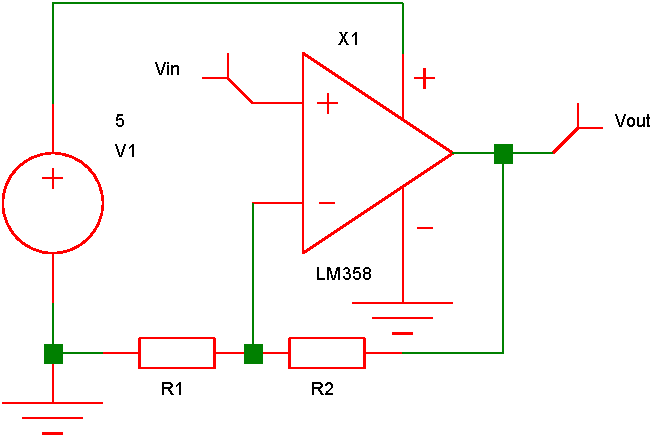
\includegraphics[width=7cm]{opamp}
\caption{Op-amp as non-inverting amplifier.}\label{fig:opamp}
\end{center}
\end{figure}

\fbox{
  \parbox{0.9\textwidth}{
    \textbf{Task: calculate $V_\text{out}$ based on $V_\text{in}$ in the non-inverting amplifier circuit shown in figure \ref{fig:opamp}. Show that for $R_2 = 0$ you obtain the voltage follower: $V_\text{out} = V_\text{in}$.}
  }
}
\vspace{0.5cm}\\
For calculations with op-amps you can use the following rules:
\begin{itemize}
\item no current flows into the two \textbf{inputs} (left side) of the op-amp. It gets all its current from the \textbf{supply} (top and bottom)
\item the op-amp puts both inputs at the same potential ("virtual-short")
\end{itemize}

After use of these two rules you can directly apply Kirchhoff's law to the circuit. 

The voltage follower circuit we build has a very high input impedance and therefore only draws very little current from the circuit with the NTC resistor. This allows us to use the formulas for an unloaded voltage-divider in the calculation and it also limits the current through the NTC, which could heat it up.

\subsection{Pulse Width Modulation (PWM)}

Pulse Width Modulation is a technique, to transmit information (or power) using a square-wave signal with fixed period and amplitude, but varying pulse-width. The fraction of time during which the signal is at the high level is called \textbf{duty cycle}. PWM signals with different duty cycles are shown in figure \ref{fig:pwm}. The frequency of the PWM signal created with \code{analogWrite()} is fixed to $\approx$ 490 Hz which is fast enough for our purpose, but it is possible to change this frequency as well, see e.g. in \cite{avrguide}.

\begin{figure}[H]
\begin{center}
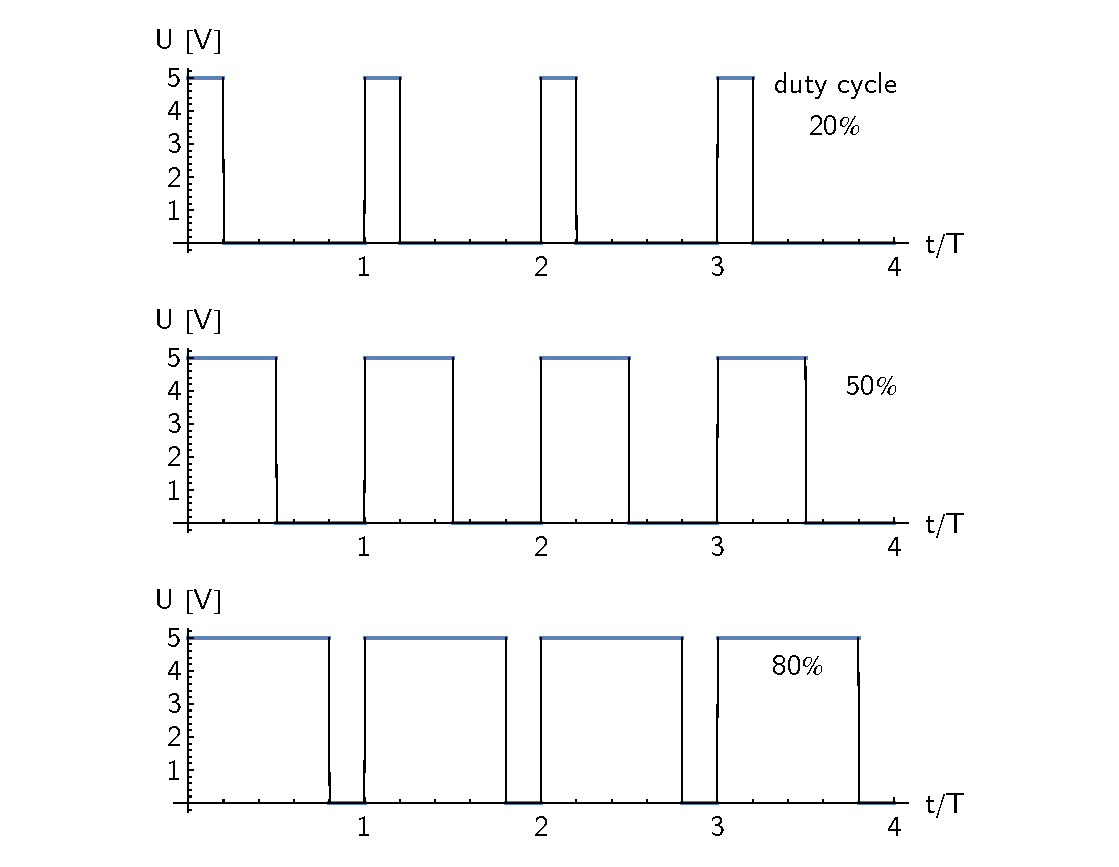
\includegraphics[width=14cm]{pwm}
\caption{PWM signals with different duty cycles 20\%, 50\% and 80\%.}\label{fig:pwm}
\end{center}
\end{figure}


\subsection{PID Controller}\label{sec:pid}
A \ac{PID} controller is a control loop feedback mechanism widely used in industrial control systems and a variety of other applications requiring continuously modulated control. A \ac{PID} controller continuously calculates an error value $e{t}$ as the difference between a desired setpoint (SP) and a measured process variable (PV) and applies a correction based on proportional, integral, and derivative terms (denoted P, I, and D respectively) which give the controller its name.\par
In practical terms it automatically applies accurate and responsive correction to a control function. An everyday example is the cruise control on a road vehicle; where external influences such as gradients would cause speed changes, and the driver has the ability to alter the desired set speed. The PID algorithm restores the actual speed to the desired speed in the optimum way, without delay or overshoot, by controlling the power output of the vehicle's engine \cite{wiki:pid}.





\section{Setup and Experimental Procedure}\label{sec:exp}
The Digital Electronics Lab is meant to be very open in implementation. The aim will be to build an automated cooling system. We will guide you through this process step by step, but you are also encouraged to bring in your own ideas of other possible implementations!

\subsection{Experimental Material}\label{sec:material}
%BEGIN Material
You will find the following objects on your test stand:
\begin{itemize}
	\item 1 Arduino Uno Board
	\item 1 Oscilloscope
	\item 2 Probes 
	\item 1 Multimeter
	\item 1 \ac{USB} Type B cable
	\item 1 Breadboard
	\item 1 Grove Starter Kit for Arduino
	\begin{itemize}
		\item 1 Base Shield
		\item 1 LCD RGB Backlight
		\item 1 Smart Relay
		\item 1 Buzzer
		\item 1 Sound Sensor
		\item 1 Touch Sensor
		\item 1 Rotary Angle Sensor
		\item 1 Temperature Sensor
		\item 1 LED Module
		\item 3 Dip LEDs (red, green, blue)
		\item 1 Light Sensor
		\item 1 Button
		\item 1 Mini Servo
		\item 10 Grove Cables
	\end{itemize}
	\item 1 3-pin fan
	\item 1 operational amplifier (\href{http://www.ti.com/lit/ds/symlink/lm158-n.pdf}{LM358})
	\item 1 NPN transistor (\href{https://www.sparkfun.com/datasheets/Components/BC546.pdf}{BC547})
	\item 1 \ac{NTC} thermistor (\href{https://eu.mouser.com/datasheet/2/400/NTC_Leaded_disks_K164-1317145.pdf}{B57164-K104-J})
\end{itemize}\vspace*{10pt}\noindent
\textcolor{red}{\textbf{In addition you should bring a lab book to note down everything what you do and measure (immediately after the execution). Please write clearly and meticulously since it will greatly help you to find mistakes and to write your report!}}
%END

\subsection{Setting up the Arduino}\label{sec:setup}
%BEGIN Arduino Setup
\subsubsection{Software installation}
We highly recommend you to install the Arduino \ac{IDE} on your machine so that you can access it any time. If you should have trouble with the installation or you prefer to not use your computer for the experiment, you can use one of the Windows XP machines provided to you, which have the Arduino IDE and all necessary drivers pre-installed. These machines do not have internet connection, so you have to bring a portable USB drive to copy the data.
\begin{itemize}
	\item install \ac{IDE} following \ar{sec:soft}
\end{itemize}

\subsubsection{Connect the Arduino}
\begin{itemize}
	\item connect the Arduino to your computer and check if it is recognised by the \ac{IDE}
	\begin{itemize}
		\item select the correct port: \fpath{Tools > Port}
		\item get board info: \fpath{Tools > Get Board Info}
	\end{itemize}
\end{itemize}

\subsubsection{Your First Sketch}
\begin{itemize}
	\item (optional) set your sketchbook location
	\begin{itemize}
		\item you can link it to your \ac{IDE}: \fpath{File > Preferences > Sketchbook Location}
	\end{itemize}
	\item create a new sketch with \fpath{File > New}, it will look like this:
\end{itemize}

\noindent\begin{minipage}{\textwidth}
\begin{lstlisting}[language=Arduino]
void setup() {
  // put your setup code here, to run once:

}

void loop() {
  // put your main code here, to run repeatedly:

}
\end{lstlisting}
\end{minipage}

Now we want to turn on the LED on the Arduino board, which is connected to the special pin \code{\var{LED\_BUILTIN}}. Since use this pin as an output, we have to set the pin mode during the \code{\meth{setup()}} function to \code{OUTPUT}. Afterwards we can use the method \code{\meth{digitalWrite()}} to set the pin to \code{\var{HIGH}}, (corresponding to 5V), which will turn on the LED on the board. We don't need to use the \code{\meth{loop()}} method for this simple sketch, but we will use it later.

\noindent\begin{minipage}{\textwidth}
\begin{lstlisting}[language=Arduino]
void setup() {
  pinMode(LED_BUILTIN, OUTPUT);
  digitalWrite(LED_BUILTIN, HIGH);
}

void loop() {
  // put your main code here, to run repeatedly:

}
\end{lstlisting}
\end{minipage}

That's it. All the methods and constants we use in this script are already defined and don't have to be imported explicitly. There is a long list of such pre-defined constants, make sure to not redefine them when adding new constants or variables!
We are now ready to test the communication of the Arduino board with the computer and test if flashing the code works. Make sure to select the correct Port and choose "Arduino/Genuino Uno" as board type if not already selected.\newline

\begin{itemize}
	\item compile the code
	\item upload the code to the Arduino
	\item add the sketch folder to a git repository
\end{itemize}

\textbf{Important: Do not use the pins A4 and A5! The Arduino Uno uses these pins for the I2C communication, which will later be used for the display! Even if it looks like they are separate pins on the shield board, they are shared internally!}


\subsection{Blinking LED on Bread Board}\label{sec:led}
%BEGIN Blinking LED
That was easy (but boring...). As next step we want to have a blinking external LED on the breadboard. Since it should continue blinking forever, we will use the \code{\meth{loop()}} function now.
\begin{itemize}
	\item supply the Breadboard with \SI{5}{\volt} from the Arduino
	\item connect a LED to the breadboard with appropriate resistor (220 Ohm) and to a digital pin
	\item write a sketch (\path{Blink.ino}) that makes the LED blink with a frequency of \SI{1}{\hertz} using the \code{\meth{delay}(int \var{nMilliSeconds})} method, which pauses the execution for \code{\var{nMilliSeconds}} milliseconds.
\end{itemize}
Upload your sketch now to the Arduino and test it.

\begin{itemize}
	\item connect a second LED on the breadboard to a different pin
	\item write a sketch (\path{Blink2.ino}) that makes the second LED blink in a different pattern than the first one
	\begin{itemize}
		\item why is \code{\meth{delay}()} not the optimal method for this task?
		\item use a timer with \code{\meth{micros}()} which returns a micro-seconds counter as \code{unsigned long}.
		\item remember to use  \code{unsigned long} to save the results of \code{\meth{micros}()}
		\item after some time (roughly 70 minutes), the 32-bit counter will overflow and start from 0 again! Make sure to handle this case well!
	\end{itemize}
\end{itemize}

\textbf{Add the code for the 2 blinking LEDs, implemented with timers, to your report.}

%END


\subsection{General tips for writing Code for the Arduino}\label{sec:codestyle}

\subsubsection{Data-types}

Data-types on Arduino are defined differently than for 32-bit or 64-bit x86 processors, e.g. \code{int} is only 16-bit, which can store values from -32768 to 32767. In most cases it's better to use \code{long} instead of int to avoid overflows. If no negative numbers are required, use \code{unsigned} versions. Note: On Arduino Uno, \code{double} and \code{float} are exactly the same.

\begin{table}[h!]\centering
	\rowcolors{2}{YellowOrange!10}{ProcessBlue!10}
	\begin{tabular}{|lll|}
		\rowcolor{PineGreen}\tline{.5}
		\bfseries
		\textcolor{white}{\textbf{type}}	&	\textcolor{white}{\textbf{length}}	& \textcolor{white}{\textbf{range}}\\\tline{1.3}
		char		&	8 bit						&	-128 to 127	\\
		unsigned char		&	8-bit		&	0 to 255	\\
		int			&	16-bit										&	-32768 to 32767	\\
		unsigned int				&	16-bit				&	0 to 65535 	\\
		long			&	32-bit										&	-2147483648 to 2147483647	\\
		unsigned long				&	32-bit				&	0 to 4294967295 	\\
		float				&	32-bit				&	floating point 	\\
		double			&	32-bit				&	floating point 	\\
		\tline{.5}
	\end{tabular}
	\caption{Basic numeric data-types for Arduino Uno.}
	\label{tab:1}
\end{table}

\vspace{0.5cm}

\fbox{
  \parbox{0.9\textwidth}{
    Be sure to use \textbf{unsigned long} to store the output of microsecond counters like \textbf{micros()}!
  }
}


\subsubsection{Avoid hard-coded values}
Instead of a hard-coded number somewhere in the middle of the program, like \newline
\noindent\begin{minipage}{\textwidth}
\begin{lstlisting}[language=Arduino]
...
if (now > lastPid + 100000) {
...
\end{lstlisting}
\end{minipage}
define a constant (with const or as macro with \#define) in the beginning of the program. Give it a systematic name, e.g. all uppercase for constants, and e.g. also include the unit (micro-seconds) here and add a comment: \newline
\noindent\begin{minipage}{\textwidth}
\begin{lstlisting}[language=Arduino]
#define INTERVAL_MICROS_PID            100000     // update interval of PID in micro-seconds
...
if (now > lastPid + INTERVAL_MICROS_PID) {
...
\end{lstlisting}
\end{minipage}
and later use this constant \code{\var{INTERVAL\_MICROS\_PID}} in the if clause. This makes the code easier to read. Macros with \code{\#define} don't use space for variables (in contrast to declaration with \code{int ...}), which reduces memory footprint of your program. Keep in mind that the total RAM is only 2 kB, which corresponds to only around 500 32-bit integers you can store and part of this is already used by libraries. Using constants instead of hard-coded numbers is especially important for pin numbers.


\subsubsection{Code documentation}
Add a short description on the functionality of your program at the top of the code. Also include the date and author name. Also comment any non-trivial steps in your code. (remember: it's generally better to write code in a self-explaining way such that no comments are necessary. Sometimes though comments are unavoidable.) \newline

\fbox{
  \parbox{0.9\textwidth}{
    \textbf{Your final code has to be added to the report. A reasonable documentation is therefore required for the report to be accepted by the assistant.}
  }
}

\subsection{Grove Temperature Sensor}\label{sec:grovetemp}
%BEGIN Grove Temp
In this experiment you will work with the \href{http://wiki.seeedstudio.com/Grove-Temperature_Sensor_V1.2/}{Grove - Temperature Sensor V1.2}. It uses a \ac{NTC} thermistor to detect the ambient temperature. The specifications are shown in \ar{tab:gt}.
\begin{table}[ht!]\centering\alternatecolors
	\begin{tabular}{|ll|}\rowcolor{PineGreen}\tline{.5}
		\fatwhite{Specification}		& \fatwhite{Value}																					\\\tline{1.3}
		Operating voltage						&	\SIrange{3.3}{5.0}{\volt}																	\\
		Zero power resistance				&	\SI{100\pm1}{\kilo\ohm}																		\\
		Operating temperature range	&	\SIrange[retain-explicit-plus]{-40}{+125}{\degreeCelsius}	\\
		Nominal $B$-constant				&	\SIrange{4250}{4299}{K}																		\\\tline{.4}
	\end{tabular}
	\caption{Grove-Temperature Sensor V1.2 specifications.}
	\label{tab:gt}
\end{table}

\begin{itemize}
	\item connect the  Shield to your Arduino
	\item connect the Grove Temperature Sensor to the shield
	\begin{itemize}
		\item figure out which connector to choose on the shield
	\end{itemize}
	\item write a sketch (\path{GroveTemp.ino}) that measures the ambient temperature
	\begin{itemize}
		\item read the voltage value from the sensor
		\item convert the voltage into the corresponding resistance
		\item convert the resistance into a temperature in \SI{}{\degreeCelsius}
		\item write the temperature to the serial interface every second
		\item look at the data with the Arduino Serial Monitor:\\ \fpath{Tools > Serial Monitor} (\code{Ctrl+Shift+M})
		\item look at the data with the Arduino Serial Plotter:\\ \fpath{Tools > Serial Plotter} (\code{Ctrl+Shift+P})
	\end{itemize}
\end{itemize}

The serial connection has to be enabled during the \code{\meth{setup()}} function with \code{Serial.begin(9600);} where 9600 is the baud rate. It is 9600 by default in the Serial Plotter and Serial monitor utilities, so it is convenient to use this.
%END


\subsection{Grove Display and Potentiometer}\label{sec:grovedisp}
%BEGIN Grove3
As a next step, we will add two more components from the Grove kit: a display to output the current temperature read by the sensor and a potentiometer to set the threshold for our two-point temperature control later. 
\begin{itemize}
    \item add the display to your project
	\begin{itemize}
        \item install the libraries from \href{http://wiki.seeedstudio.com/Grove-LCD_RGB_Backlight/}{http://wiki.seeedstudio.com/Grove-LCD\_RGB\_Backlight/}
        \item look at the example code on the above website, especially on how to include the libraries in your project and how to initialize it during the \code{setup()} routine
        \item make sure the "3V3\_VCC\_5V" switch on the Grove shield is set to 5V, otherwise the display will not work correctly
	    \item connect the Grove LCD RGB Backlight display to your Grove shield
		\item modify your project such that the measured temperature is printed on the display every second 
	\end{itemize}
	\item define a fixed threshold in your code, e.g. 30 degrees above which a LED is turned on. (As alternative you can change the background color of your display). Test if your project is working.
	\item now we want to make the threshold controllable without recompiling our project. For this purpose, connect the potentiometer (Grove Rotary Angle Sensor) to the Grove shield (you can also use the sliding potentiometer instead if you prefer)
	\begin{itemize}
        \item read the description at \href{http://wiki.seeedstudio.com/Grove-Rotary_Angle_Sensor/}{http://wiki.seeedstudio.com/Grove\-Rotary\_Angle\_Sensor/}
        \item read-out the sensor with \code{analogRead()}
        \item to map the ADCs which range from 0 to 1023 to a reasonable temperature range (a, b), e.g. 20 to 40 degrees, the function \code{map(degrees, 0, 1023, a, b)} can be used for convenience
 	\end{itemize} 
 	\item indicate the status below/above threshold also in the output to the serial interface, e.g. add a second number (0 = below threshold, 50 = above threshold) separated by a space
    	\item test your code by varying the threshold below/above the room temperature
	\begin{itemize}
		\item the serial plotter should now draw a second line indicating whether below or above threshold. Vary your threshold slowly below and above the room temperature and make a screenshot of the resulting graph.
 	\end{itemize}
    	\item optional: while turning the potentiometer, you can also print the threshold temperature on the display in the second row below the measured temperature
\end{itemize}

\textbf{Don't forget to add the code for this exercise to your report!}
%END

\subsection{Data Handling}\label{sec:data}
%BEGIN Data Handling
Even though one can use the Arduino \ac{IDE} to look at the values from the temperature sensor, there is no way to save them. That is why we encourage you to write a short program to save the data to file so that you can use it afterwards. We recommend you to use python for this purpose, but feel free to use whatever you have the most experience with. The easiest solution for Windows is the "type" command, which is explained below. \par
Once a sketch is uploaded to the microprocessor the Arduino will perform the loop until it is disconnected from power or overwritten by a new sketch. Note down the port number or name, which can be seen under "Tools" in the Arduino IDE. In order to read the data externally from the serial port you have to close the Arduino serial tools (Serial Monitor, Serial Plotter, ...).\\


\subsubsection{With Python}

Python needs the \textbf{pyserial} package to be able to read from the serial interface.


\noindent If you are using \textbf{anaconda}, type the following command in your anaconda shell:
\begin{lstlisting}[language=bash]
  conda install -c anaconda pyserial
\end{lstlisting}

\noindent If you are using \textbf{pip}:
\begin{lstlisting}[language=bash]
  pip install pyserial
\end{lstlisting}


You can test if you have installed the \textbf{pyserial} package correctly by typing "import serial" into a Python shell. After this works, you can start writing you Python code. An outline of what the code should do is below:
\begin{itemize}
	\item open the serial port
	\begin{itemize}
		\item \code{\var{from} serial \var{import} Serial}
		\item \code{arduino = Serial(\str{'/dev/<arduino\_portname>'})}
		\item you can find the name of the port in the Arduino \ac{IDE}
		\item read a single line using the serial method \code{arduino.readline().decode('utf-8')}  
	\end{itemize}
	\item print the line in the terminal using \code{print}
	\item write the data to a text file (\path{data.txt}), every value on a single line
	\begin{itemize}
		\item if you have trouble handling files in python follow this \href{http://www.pythonforbeginners.com/files/reading-and-writing-files-in-python}{guide}
	\end{itemize}
	\item your program should repeat this until you terminate it e.g. by pressing CTRL+C.
	\item optional: add timestamps to every line in your log-file. This makes it easier later analyze the data.
\end{itemize}

On Windows, the Arduino is typically called "COM3", so do \code{arduino = Serial("COM3")} to open it.

\subsubsection{On Windows XP lab computers}

If your port is COM3, you can type the following simple command into a command shell (Start > Run > cmd):

\begin{lstlisting}
type com3: > output.log
\end{lstlisting}

There is a small delay in writing as data is written in blocks. It can also happen that the last line is incomplete, take this into account in the analysis of the file. You can stop the program by pressing CTRL+break in the command shell. You can use a USB stick to transfer the resulting file to your personal computer to proceed with the analysis.

\subsubsection{bash (Linux, Mac OSX}
If you use Linux or Mac, you can do all of the above with a single line of bash. Instead of "/dev/cu.usbmodem14141" put your device name (which is listed as port in the Arduino IDE), which can be different from this.

\begin{lstlisting}
while read -r line; do echo $line; 
    done < /dev/cu.usbmodem14141 | tee "output.txt"
\end{lstlisting}



\subsection{Op-Amp Circuit}\label{sec:temp}
%BEGIN Temperature Sensor
In this task you will build your own temperature sensor using an B57164-K104-J NTC resistor and LM358 Op-amp. The \href{https://eu.mouser.com/datasheet/2/400/NTC_Leaded_disks_K164-1317145.pdf}{B57164-K104-J} thermistor has the specifications listed in \ar{tab:ts}.
\begin{table}[ht!]\centering\alternatecolors
	\begin{tabular}{|ll|}\rowcolor{PineGreen}\tline{.5}
		\fatwhite{Specification}		& \fatwhite{Value}																					\\\tline{1.3}
		Operating voltage											&	\SIrange{3.3}{5.0}{\volt}																	\\
		Zero power resistance				&	\SI{100\pm5}{\kilo\ohm}																		\\
		Operating temperature range	&	\SIrange[retain-explicit-plus]{-55}{+125}{\degreeCelsius}	\\
		Nominal $B$-constant				&	\SI{4600\pm138}{K}																		\\\tline{.4}
	\end{tabular}
	\caption{B57164-K104-J specifications.}
	\label{tab:ts}
\end{table}

\begin{itemize}
	\item build a voltage divider circuit to convert the resistance into a measurable voltage
	\item use the LM358 operational amplifier (as voltage follower with gain 1) to amplify the sensor signal. The pin layout is given in the datasheet or in figure \ref{fig:tempcircuit2}.
	\item reproduce the temperature measurements from \ar{sec:grovetemp}
\end{itemize}

\begin{figure}[H]
\begin{center}
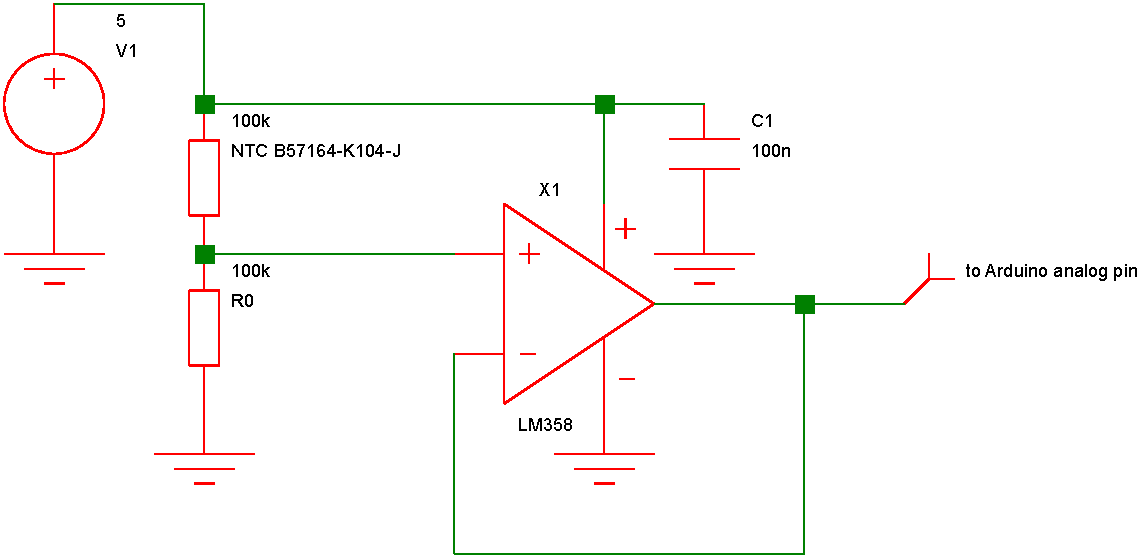
\includegraphics[width=14cm]{ntc_opamp_schematic}
\caption{Circuit for reading the NTC resistance with Op-amp.}\label{fig:tempcircuit}
\end{center}
\end{figure}

Figure \ref{fig:tempcircuit} shows the simplest possible circuit you can use for this purpose. The high input impedance of the op-amp ensures that there is basically no load on the voltage divider and we can use the simple formula which is only valid without load. There is then also virtually no current flowing through the NTC resistor which would heat it up.


\begin{figure}[H]
\begin{center}
  \centering
  \begin{minipage}[b]{0.4\textwidth}
    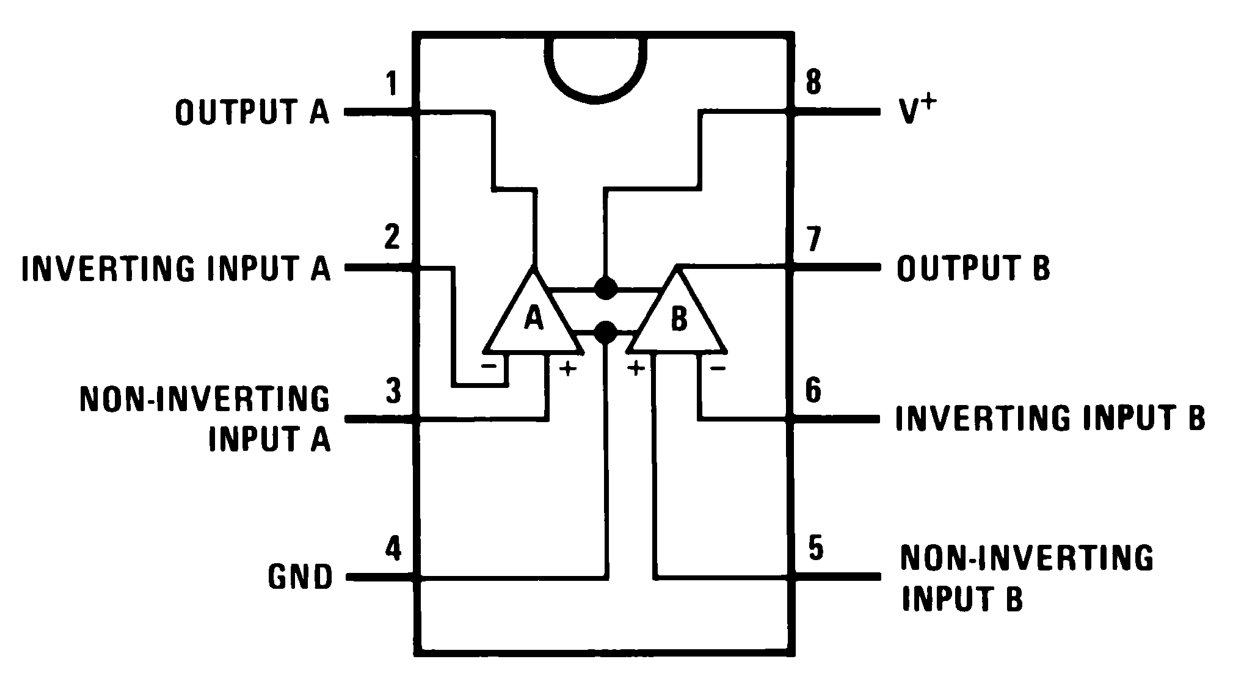
\includegraphics[width=\textwidth]{lm358pins}
  \end{minipage}
  \hfill
  \begin{minipage}[b]{0.5\textwidth}
    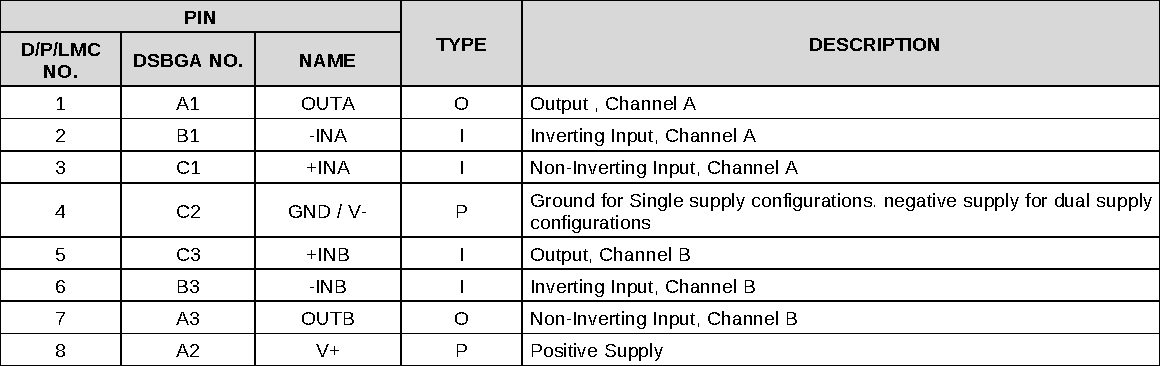
\includegraphics[width=\textwidth]{lm358table}
  \end{minipage}
\caption{Pin layout (left) and descriptions (right) of the LM358 Op-Amp. Source: datasheet from http://www.ti.com/lit/ds/symlink/lm158-n.pdf}\label{fig:tempcircuit2}
\end{center}
\end{figure}


\subsection{Calibration}\label{sec:calibration}

The NTC resistor we used for this experiment is not calibrated yet and therefore we obtain a relatively large error on the absolute temperature scale.
\vspace{0.5cm}
\begin{center}
\fbox{
  \parbox{0.9\textwidth}{
    \textbf{Task: calculate the uncertainty on the temperature we obtain from the following sources:}
    \begin{itemize}
    		\item B-constant of the NTC
    		\item resistance of the 100 k resistor (use 1\% resistors if possible)
    		\item resolution of the ADC
    		\item any other non-negligible uncertainty you find
    \end{itemize}
  }
}
\end{center}

By calibrating our device with an already calibrated reference device, we can reduce the systematic uncertainties. For this calibration we can use the Sensirion SHT21 temperature sensor or any equivalent device.

\vspace{0.5cm}
\begin{center}
\fbox{
  \parbox{0.9\textwidth}{
    \textbf{Task: calibrate your device by adjusting the B constant, such that its measured temperature matches the one measured with the reference device. Use the given uncertainty on the temperature of the reference device to calculate a new uncertainty for your B constant. How much does it improve?}
}
}
\end{center}


%END

\subsection{Heating}\label{sec:heat}
Since it is boring to measure a constant temperature, we build a simple heat load of 0.2-0.25 W with a couple of resistors.
\begin{itemize}
	\item calculate the resistors needed to have the correct power dissipation.
	\item bring the heating resistor and the temperature sensor close together to have as good thermal contact as possible.
\end{itemize}

Important: the temperature difference between the room temperature and the equilibrium temperature without cooling should be at least 5 degrees, better more (e.g. 10). 
If improving the thermal contact is not enough to heat up the NTC to more than 5 degrees above the room temperature, use the external power supply to provide power for the heating resistor.

\vspace{0.2cm}
\begin{center}
\fbox{
  \parbox{0.9\textwidth}{
    \textbf{Task: create a plot of the temperature vs. time (starting from room temperature) and determine the time constant of the temperature rise and estimate the equilibrium temperature from a fit.}
  }
}
\end{center}
\vspace{0.2cm}

\subsection{Cooling}\label{sec:cool}
Many electrical components will produce heat under load and may break at critical temperatures. That is why many of complex systems like computers require cooling. You will now build a system that controls a fan and can regulate it's rotation speed.
\begin{itemize}
	\item connect the fan to the breadboard, for the 4 pin header, the following conventions are used:
	\begin{itemize}
	    \item black: ground
	    \item yellow: 5V
	    \item green: tacho read-out (will be used later)
	    \item blue: PWM control
	\end{itemize}
	\item keep in mind that only a few of the digital pins (marked by "{\raise.17ex\hbox{$\scriptstyle\sim$}}" on the board) are able to use PWM, e.g. use digital pin 11
\end{itemize}

\subsection{Two-point controller}\label{sec:cool2}
Now we can finally build the full two-point controller.
\begin{itemize}
    \item define a low and high threshold, e.g. use the potentiometer for the high threshold and set the lower threshold a few degrees lower than the high one. both thresholds have to be in reach
	\item set the duty cycle of the fan to 100\% when above the high threshold
	\item set the duty cycle of the fan to 0\% when below the low threshold
	\item setting the PWM duty-cycle can be done using the \code{analogWrite()} function
\end{itemize}
Experiment with different set-points. What is the advantage of having two setpoints instead of a single threshold above we turn cooling on? What are the draw-backs of the two-point controller?

\vspace{0.5cm}
\begin{center}
\fbox{
  \parbox{0.9\textwidth}{
    \textbf{Task: create a plot of temperature vs. time with the two-point controller active which shows multiple periods.}
  }
}
\end{center}

\subsection{Read Out the Fan Speed}
We now wan to use the built-in Hall Effect Sensor (HES) of the fan to measure its rotation speed. In every rotation this sensor will produce two pulses we can count and then convert to revolutions per minute (\textbf{RPM}). The maximum (for 100\% duty cycle) according to the datasheet is 1900 RPM, with a tolerance of 10\%, the minimum is around 230 RPM.

\begin{itemize}
	\item calculate a rough estimate for the minimum frequency needed for reading the voltage on the tacho pin and be able to count the pulses? (Use Nyquist theorem) In practice, a much higher frequency should be used than the limit calculated above
	\item check the Arduino reference of \code{analogRead()} for the maximum frequency. Since we also have to do other work in the \code{loop()} function, the frequency should be also much less than the maximum. Make a reasonable choice.
    \item what is the expected uncertainty on the minimum and maximum RPM if we count pulses for 1 second?
	\item connect the tacho (green wire) of the fan to an analog pin of the Arduino, using a 10k pull-up resistor to 5V. (optional: figure out how to use internal pull-up resistor of the Arduino instead of a discrete component)
	\item what is the role of the pull-up resistor?
	\item count the pulses of the HES and convert the result to RPM. Is it within the range expected by the datasheet numbers?
	\item write the \ac{RPM} value to the serial output
\end{itemize}

\vspace{0.1cm}
\begin{center}
\fbox{
  \parbox{0.9\textwidth}{
    \textbf{Task: plot the fan RPM vs. the duty cycle. Which is the minimum duty cycle above which the fan starts to spin, and at which RPM? What is the maximum RPM for full duty-cycle?}
  }
}
\end{center}
\vspace{0.5cm}

Scanning the points for the different duty cycles should be done without flashing the device in between. Instead, the measurement programme (e.g. number of steps, seconds per step etc.) should be programmed into the Arduino or, alternatively, controlled by a Python program running on the computer which changes the parameters via the serial interface (see "Bi-directional communication with the computer" section below).

\subsection{Equilibrium temperature}
\begin{center}
\fbox{
  \parbox{0.9\textwidth}{
    \textbf{Task: plot the equilibrium temperature vs. the fan RPM. Make sure you measure long enough for each data point and give a reasonable estimate for the uncertainty that you obtain on the equilibrium value.}
  }
}
\end{center}
\vspace{0.5cm}

It might need few minutes to reach a stable equilibrium per point.


\subsection{PID Controller}
We have seen that with the two-point controller above, we could not exactly stabilize to a constant temperature and were suffering from under- and overshoot. Using a \ac{PID} controller can overcome both issues.
\begin{itemize}
	\item implement a \ac{PID} controller
	\item regulate cooling by the PWM duty-cycle of your fan
	\item tune your three parameters to have reasonably stable operation. (Perfect tuning is very complicated and does not have to done here.)
	\item create some plots with temperature vs. time, starting from different initial temperatures, which show converging temperature.
\end{itemize}

The output of the PID controller consists of three different terms, each having a tuneable coefficient.
\begin{itemize}
	\item proportional: proportional to the error, which is \code{error = temperature - setpoint}
	\item integral: proportional to the sum of all errors of previous steps
	\item derivative: proportional to the difference in error compared to last step
\end{itemize}

In practice, there are few more things to consider
\begin{itemize}
    \item using a timer, perform the PID calculations between every 100 ms and every second. You should not use longer values to be fast enough in response and not too much shorter values to be not susceptible to noise.
    \item use a discrete digital low-pass filter on your measured temperature if it is noisy.
    \item convert your PID response to a duty\_cycle between 0 and 255 to be used in \code{\meth{analogWrite}(\var{PIN\_FAN\_PWM}, duty\_cycle)}. 
\end{itemize}

\begin{center}
\fbox{
  \parbox{0.9\textwidth}{
    \textbf{Task: Optimize the three parameters reasonably well to have fast convergence and low fluctuations after a certain time and plot the temperature vs. time. Also de-tune your parameters to produce slow convergence and/or overshooting/oscillations and show both curves in one plot.}
  }
}
\end{center}

\vspace{0.5cm}

A low-pass filter can be used to filter out high frequency fluctuations (noise) on the measured temperature. It can be implemented in it's simplest form with

\noindent\begin{minipage}{\textwidth}
\begin{lstlisting}[language=Arduino]
temperature = (1-LOWPASS_ALPHA) * temperature + LOWPASS_ALPHA * temperature_current;
\end{lstlisting}
\end{minipage}

where \code{temperature\_current} is the actual reading from the sensor and \code{temperature} (which has to be properly initialized once to be the sensor reading!) the output of the filter. \code{\var{LOWPASS\_ALPHA}} and the interval between two measurements $\Delta t$ control the cut-off frequency of the lowpass filter. Set it to a reasonable value which suppresses the noise and is still fast enough for the timescale of temperature changes we expect (order of few degrees per second). It can also be computed analytically:

\begin{equation}
\alpha = \frac{\Delta t}{\tau + \Delta t}
\end{equation}

where $\tau$ is the characteristic time constant of the low-pass filter (corresponds to RC time of a RC filter). Setting $\alpha = 0$ makes it infinitely fast, so the output is equal to the input, where as $\alpha = 1$ makes the response infinitely slow, so the output would stay constant at its initial value.

\subsection{Advanced tasks}

\fbox{
  \parbox{0.9\textwidth}{
    \textbf{All of the following tasks are optional. They can be used to replace some of the other tasks if agreed on with the assistant.}
  }
}


\subsection{Fit heating/cooling(Advanced)}
Take the two-point controller and set the two setpoints far from each other, but still in achievable range. For heating and cooling process, find a suitable function to describe the data and perform a fit of the model to data. List the fit parameters (with uncertainties!) and repeat this for several cycles. Take special care on correlation of input uncertainties in the fit and explain in the report why this is an issue here and what effect it would have to neglect correlations. Also look at the uncertainties and correlations of the fitted parameters.
Are the uncertainties obtained by repeating the experiment consistent with the uncertainties from the fit? If not discuss why.

\subsection{Bi-directional communication with the computer (Advanced)}
Until now we only read values from the device, but we can also write commands from the computer to the Arduino using the serial interface.
\begin{itemize}
	\item instead of using the potentiometer to set the threshold, implement a way to set the threshold via serial commands
	\item one can use the SCPI protocol as a reference, e.g. set the threshold to 32 degrees with the command "SET:THR 32"
	\item which other commands are necessary to run the measurements from above section without hardcoding the measurement programme (e.g. number of steps, seconds per step etc.)?
	\item write a Python script to perform the measurements from above section via sending SCPI style commands to the Arduino
\end{itemize}


\subsection{Use of other components (Advanced)}
There is also a bunch of other components available which can be used to extend your Arduino project. Among them:
\begin{itemize}
	\item ultra-sonic distance sensor
	\item electric current sensor
	\item infrared leds and sensor
	\item electro magnet
	\item Piezzo vibration sensor
	\item 96x96 pixels OLED display
	\item Servo motor
	\item ...
\end{itemize}

Ask the assistants for more information if you are interested in using them. For example you could use the distance sensor and servo motor to keep an object at a fixed position relative to another moving one.


\subsection{I2C protocoll debugging (Advanced)}
Many of the Grove components communicate via I2C bus protocol. Using a digital oscilloscope, it is possible to look at the I2C signal and manually decode it on the scope. Use the Grove RBG LCD display, initialize it and periodically write text to the display and set the color. Spy on the commuication, find out the the device IDs of the 2 devices connected to the bus. What do they correspond to? Compare with the library of the Grove display. Record a short communication of a few bytes and decode it.
















\section{Analysis \& Report}

The analysis and the following report should be done if a fashion, that the reader is able to reconstruct the described circuits and is able to proof that it is working correctly. Besides the exact description of all the used parts, this includes:
%
\begin{itemize}
  \item A link to the git repository with all the used sketches. The code should be written in a readable fashion according to \href{https://gist.github.com/lefticus/10191322}{\cpp coding guidelines} with meaningful denotations and sufficient comments.
  \item The circuit diagrams of \textcolor{red}{\textbf{ALL}} circuits. A circuit diagram consists of international standardised symbols for all parts in the circuit. You can, of course draw the diagrams manually, but there are also handy tools for that, like  \eg fritzing \cite{fritz}.
\end{itemize}
%
In addition, you should answer all questions posed in \ar{sec:exp} and describing the approach on solving them. Do not forget to add a results and a conclusion section!\par
%
If need help displaying code, or just like the style of this manual, have a look at the \TeX~source code \cite{man}.












% --------------------------- BACKMATTER --------------------------------------
\newpage
\pagenumbering{Roman}
\listoffigures
\listoftables
\newpage
\section*{List of Acronyms}
\begin{acronym}[Bash]
	\acro{IDE}{integrated development environment}
	\acro{DIY}{do-it-yourself}
	\acro{USB}{Universal Serial Bus}
	\acro{I/O}{input/output}
	\acro{GND}{ground}
	\acro{RST}{reset}
	\acro{PWR}{power}
	\acro{IC}{integrated circuit}
	\acro{PCB}{printed circuit board}
	\acro{VCC}{voltage common collector}
	\acro{OS}{operating system}
	\acro{PTC}{positive temperature coefficient}
	\acro{NTC}{negative temperature coefficient}
	\acro{ADC}{analogue-to-digital converter}
	\acro{BJT}{bipolar junction transistor}
% 	\acrodefplural{ROCs}{readout chips}  
\end{acronym}
\newpage
\bibliographystyle{plain}
\bibliography{backmatter/refs}
%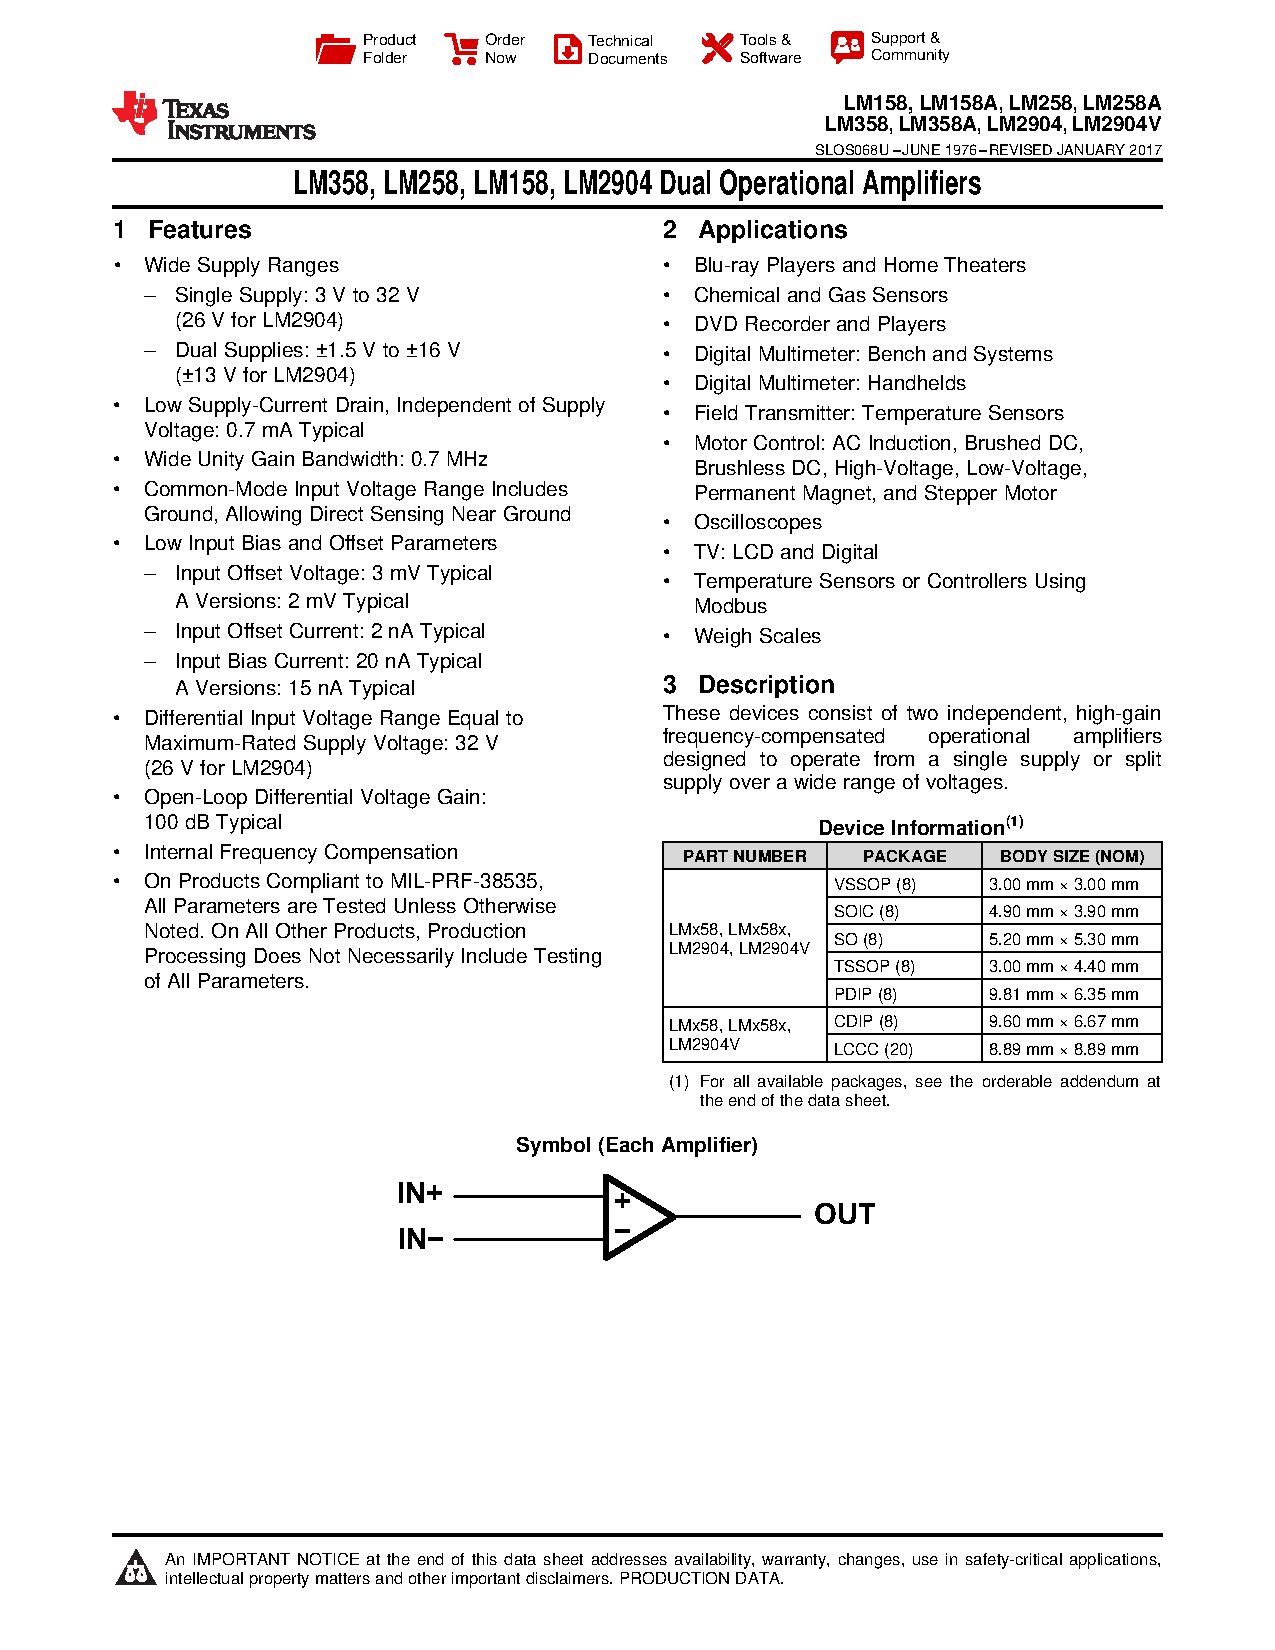
\includepdf[pages=-]{LM358.pdf}
%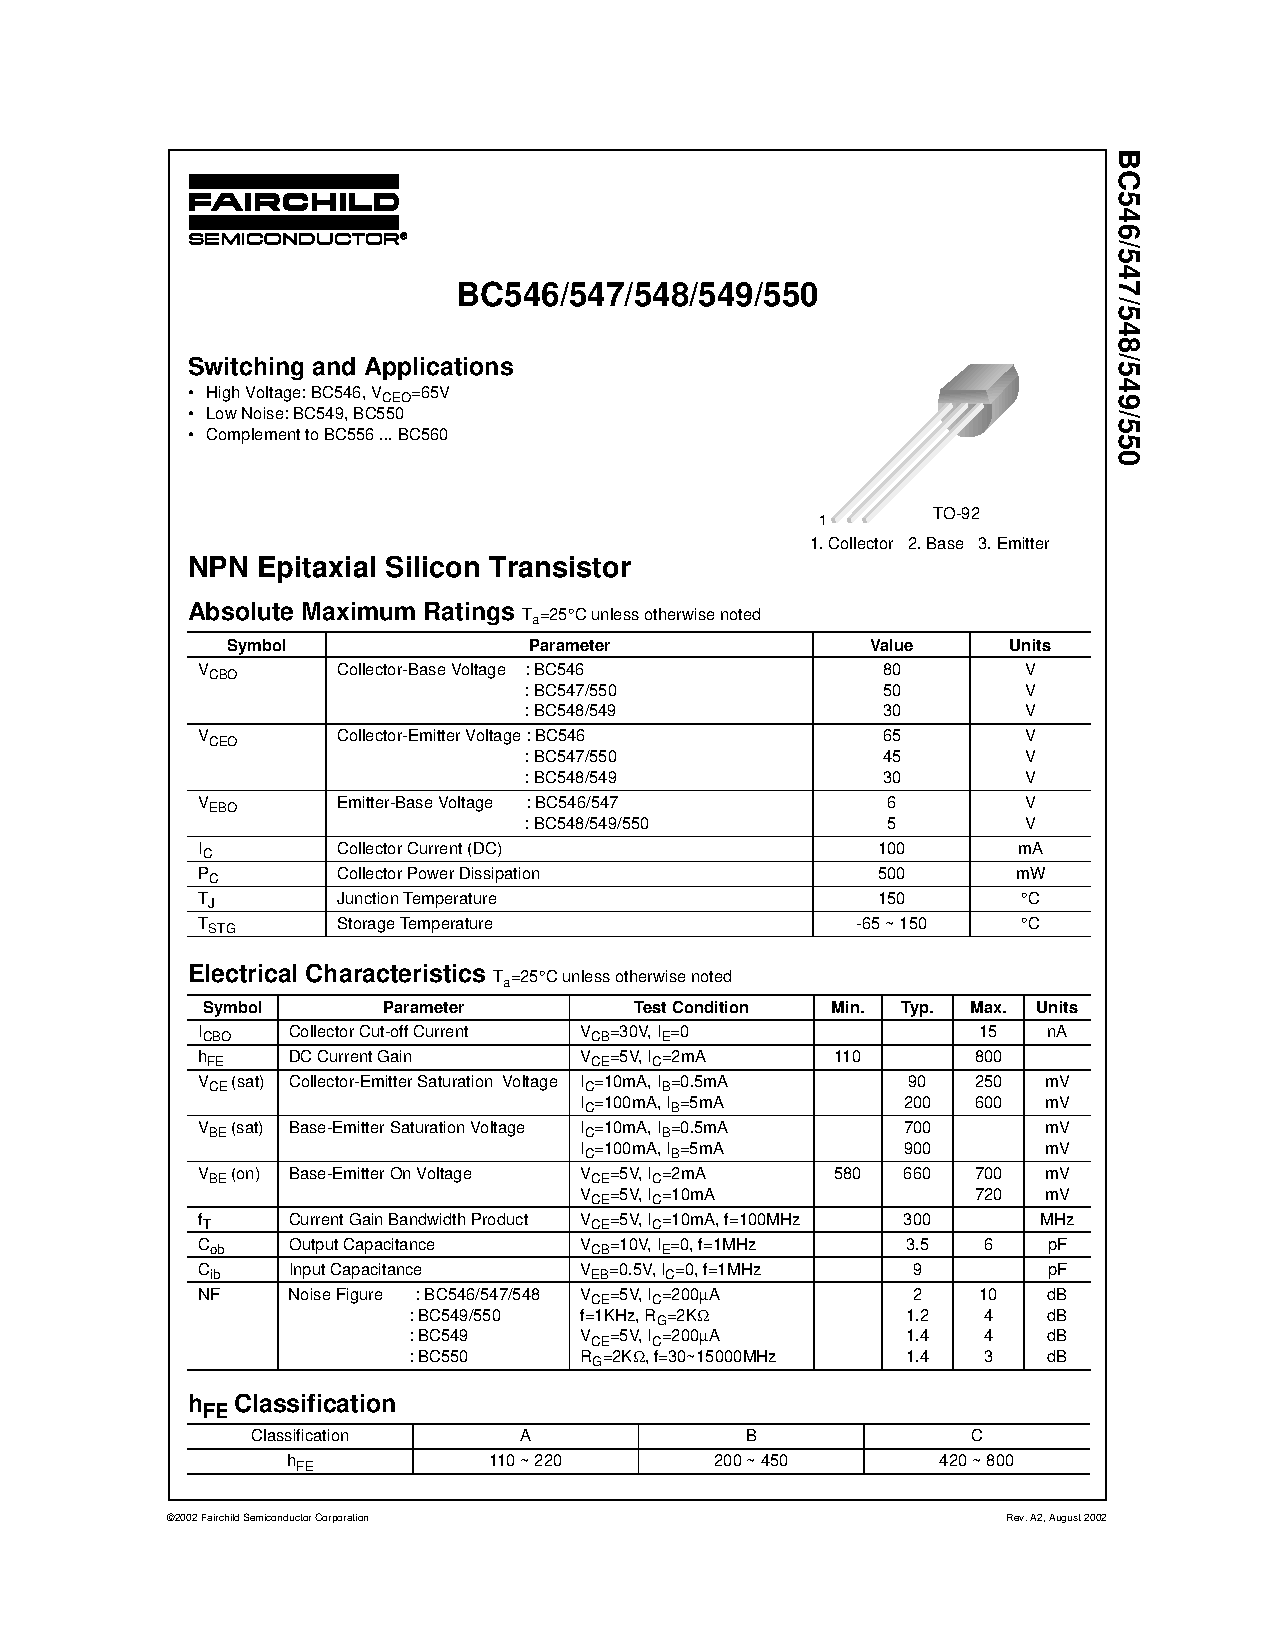
\includepdf[pages=-]{BC547.pdf}


\end{document}
